%\documentclass[aspectratio=169,handout]{beamer}
\documentclass[10pt, aspectratio=169]{beamer}
\usepackage[french,noconfigs]{babel}
\usepackage{beamerx}
  \setbeamercovered{invisible}
\usepackage{jonas}


% \graphicspath{{fig/}{fig/beamerx/}}
% \newcommand*\InputTable[1]{\input{fig/#1}}
\graphicspath{{fig/}{fig/beamerx/}{../me/all-reports/higgsstrahlung_inclusive/fig/}}
\newcommand*\InputTable[1]{\input{fig/#1}}


\title[ILD Analysis/Software Meeting]
  {\texorpdfstring{{$\nu\bar{\nu}H$}}{vvH}: My first steps with\\the 2020 MC sample}
      [vvH: DBD vs MC2020]
\author[Jonas Kunath]{Jean-Claude Brient, \emph{Jonas Kunath} (LLR)}
\date{09.12.2020}%{\today}

\begin{document}
  \maketitle
  \newcommand{\outline}{
  % <beamer> ToC only shown in beamer mode: avoid all the ToCs for handout.
  \begin{frame}<beamer>[noframenumbering]
    \frametitle{Outline}
    \begin{columns}[c,onlytextwidth]
      \begin{column}{0.6\textwidth}
        \tableofcontents[currentsection]
      \end{column}
      \begin{column}{0.4\textwidth}
        \textbf{\color{llblue}Disclaimer:}\\
        Most differences probably originate in my incomprehension.
        \newline\newline
        \url{https://github.com/kunathj/ILD_vvH_DBD_vs_MC2020}
      \end{column}
    \end{columns}
  \end{frame}
}
\newcommand{\handoutline}{
  \begin{frame}[noframenumbering]
  %\begin{frame}<handout>[noframenumbering]
    \frametitle{Outline}
    \begin{minipage}{.9\paperwidth}\noindent\center
      \Large $\nu\bar{\nu}H$: My first steps with the 2020 MC sample
    \end{minipage}
    \vfill
    \begin{columns}[c,onlytextwidth]
      \begin{column}{0.4\textwidth}
        \textbf{\color{llblue}Disclaimer:}\\
        Most differences probably originate in my incomprehension.
        \newline\newline
        \url{https://github.com/kunathj/ILD_vvH_DBD_vs_MC2020}
      \end{column}
      \begin{column}{0.5\textwidth}
        \tableofcontents
      \end{column}
    \end{columns}
  \end{frame}
}\handoutline % \outline or \handoutline.
  \xsection{myblue}{Research question}

\begin{frame}
  \frametitle{$g_{HZZ}$ - What can be gained?}
  Extracted from Higgsstrahlung events at a $\sqrt{s}=250$~\GeV.
  \begin{columns}[c,onlytextwidth]
  \begin{column}{0.60\textwidth}
  \begin{itemize}
    \item $Z \rightarrow \mu^+ \mu^-, Z \rightarrow e^+ e^-$:
          Golden channels.

          Recoil mass method, already {\color{llblue}
            \href{https://arxiv.org/abs/1604.07524}{studied elsewhere.}}
    \item $Z \rightarrow \tau^+ \tau^-$:
        Tagging on the $\tau$ is complicated.
        \begin{itemize}
          \item Large $\tau$ decay opening angle (low $E_\tau$).
          \item Divers environment from the Higgs decay.
        \end{itemize}
    \item $Z \rightarrow \nu\bar{\nu}$:
      \begin{itemize}
        \item[--] Significant WW-fusion contribution in $\nu\bar{\nu}H$.
        \item[--] Cannot tag event on $\nu$.
        \item[+]  Only Higgs boson (and beam overlay)

            present in event.
        \item[+]  $6\times$ higher cross section.
      \end{itemize}
  \end{itemize}
  \end{column}
  \begin{column}{0.40\textwidth}
    \resizebox{\textwidth}{!}{
      % Define styles for the different kind of edges in a Feynman diagram
\tikzset{
    vector/.style={decorate, draw=black,
    decoration={snake, segment length=4mm, amplitude=1mm}},
    fermion/.style={draw=black, postaction={decorate},
        decoration={markings,mark=at position .55 with {\arrow[draw=black]{>}}}},
    fermionbar/.style={draw=black, postaction={decorate},
        decoration={markings,mark=at position .55 with {\arrow[draw=black]{<}}}},
    gluon/.style={decorate, draw=black,
        decoration={coil,amplitude=4pt, segment length=5pt}},
    higgs/.style={dashed,draw},
    photon/.style={decorate, decoration={snake}, draw=black},
    electron/.style={draw=black, postaction={decorate},
        decoration={markings,mark=at position .55 with {\arrow[draw=black]{>}}}},
    positron/.style={draw=black, postaction={decorate},
        decoration={markings,mark=at position .55 with {\arrow[draw=black]{<}}}}
}


\begin{tikzpicture}[line width=1.5pt, scale=1]
    \node (i1 e+) at (-140:2) {};
    \node (v4 ISR) at (-140:1.5) {};
    \begin{scope}[shift={(v4 ISR)}]
        \node (f4 gamma) at (10:1.5) {};
    \end{scope}
    \node (i2 e-) at (140:2) {};

    \node (v1 eeZ) at (0,0) {};
    \node (v2 ZZH) at (0:2) {};
    \begin{scope}[shift={(v2 ZZH)}]
        \node (v3 Zll) at (-40:1.5) {};
        \node (f1 H) at (40:1.6) {};
    \end{scope}
    \begin{scope}[shift={(v3 Zll)}]
        \node (f3 l-) at (-60:2) {};
        \node (f2 l+) at (-20:2) {};
        \node (v5 FSR) at (-20:0.5) {};
    \end{scope}
    \begin{scope}[shift={(v5 FSR)}]
        \node (f5 gamma) at (0:1.5) {};
    \end{scope}
    \begin{scope}[shift={(f3 l-)}]
        \node (f6 nu tau) at (-10:1.5) {};
        \node (f7 W) at (10:1.5) {};
    \end{scope}

    
    \draw[fermionbar] (i1 e+)--(v1 eeZ.center);
        \node at (i1 e+) {$e^+$};
    \draw[fermion] (i2 e-)--(v1 eeZ.center);
        \node at (i2 e-) {$e^-$};

    \draw[vector] (v1 eeZ.center)--(v2 ZZH.center);
        \node at ($ 0.5*(v1 eeZ) + 0.5*(v2 ZZH)  + (0,0.3) $) {$Z$};
    \draw[vector] (v2 ZZH.center)--(v3 Zll.center);
        \node at ($ 0.5*(v2 ZZH) + 0.5*(v3 Zll)  + (0.2,0.2) $) {$Z$}; % = midpoint of propagator + fine tuning	
    \draw[higgs] (v2 ZZH.center)--(f1 H);
        \node at (f1 H) {$H$};	

    \draw[vector] (v4 ISR.center)--(f4 gamma);
    \node at (f4 gamma) {$\gamma$};

    \draw[fermion] (v3 Zll.center)--(f3 l-);
    \draw[fermionbar] (v3 Zll.center)--(f2 l+);

    \node at (f3 l-) {$f$};
    \node at (f2 l+) {$\bar{f}$};    
    
\end{tikzpicture}
    }
  \end{column}
  \end{columns}
  \end{frame}


\begin{frame}
  \frametitle{\texorpdfstring{{$\nu\bar{\nu}H$}}{vvH}}
  \begin{columns}[c,onlytextwidth]
  \begin{column}{0.55\textwidth}
  \begin{itemize}
    \item $\sigma_{\nu\bar{\nu}H}$ with contributions from both Higgsstrahlung
        and WW-fusion.
    \item Their relative size varies with the beam polarisation.
    \item Similar distributions for $\sqrt{s}=250~\GeV$.
    \item Idea: Extract the combined cross section

        ($\rightarrow$ production mode agnostic selection).
    \item WIP: Determine the benefit of this observable for $G_{HZZ}, G_{HWW}$
        from a global fit, including the correlations with e.g.
        $\sigma_{\tn{WW-fusion} \rightarrow \nu\bar{\nu} b\bar{b}}$

        (using {\color{llblue}\href{https://arxiv.org/abs/1706.02174}{SFitter}}).
  \end{itemize}
  \end{column}
  \begin{column}{0.45\textwidth}
  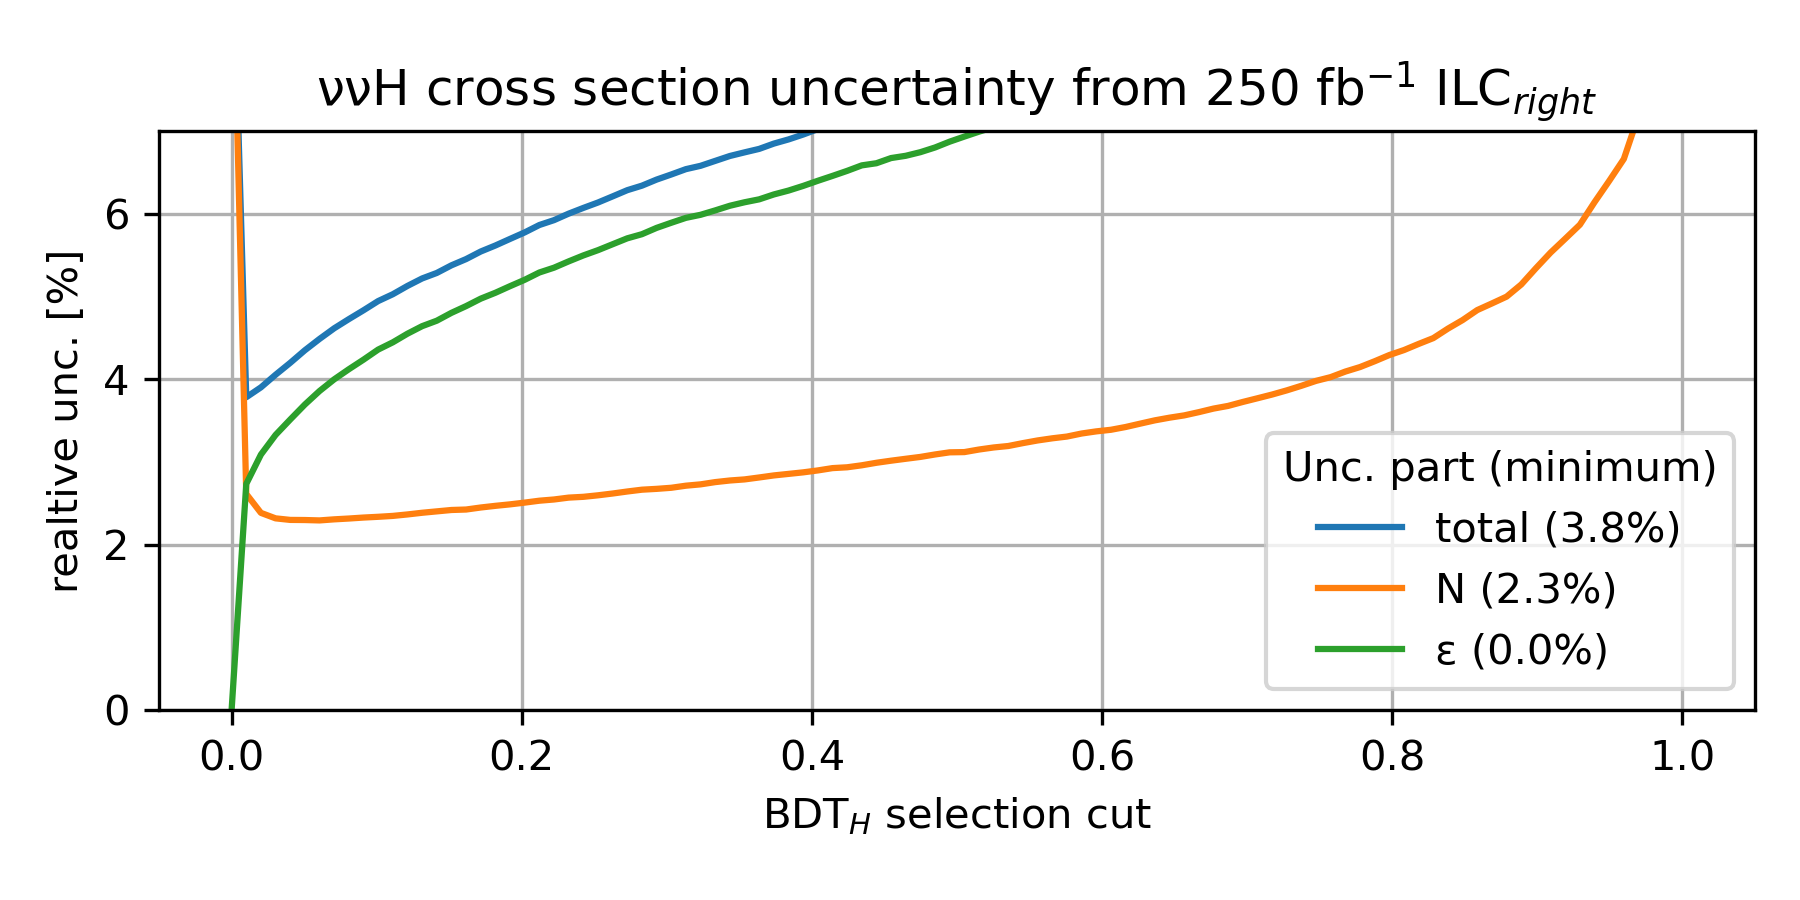
\includegraphics[height=0.5\textheight, width=0.8\textwidth, keepaspectratio]
      {ext_nnH_cs_uncertainty}
  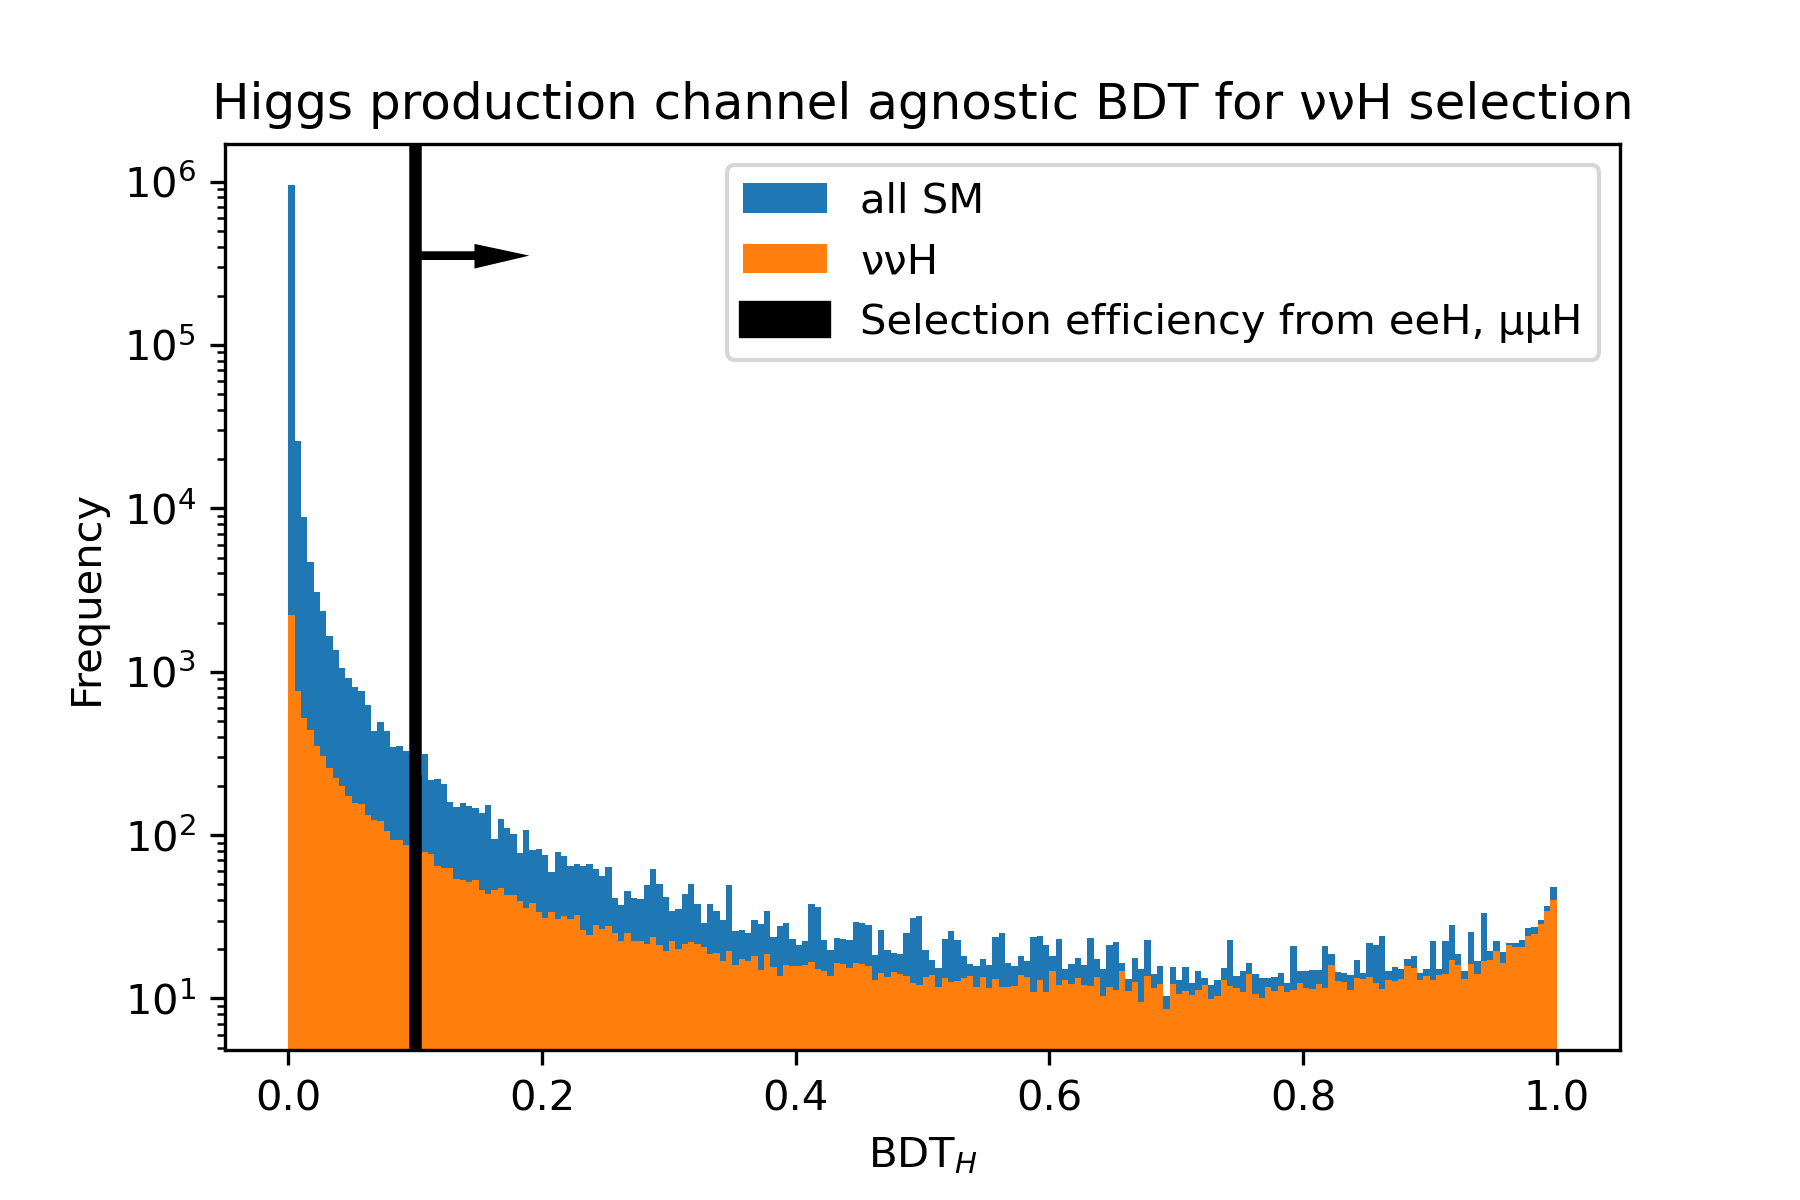
\includegraphics[height=0.7\textheight, width=\textwidth, keepaspectratio]
      {ext_nnH_BDT_production_agnostic}
  \end{column}
  \end{columns}
  \end{frame}
  \xsection{myblue}{Expectations \& getting started}

\begin{frame}
  \frametitle{Expectations}
  \begin{itemize}
    \item Smoother distributions due to increases sample size
        ($\times 10~\nu\bar{\nu}H$, $\times 60~\mu^+\mu^- H$).
    \item Great improvement for  rare (Higgs decay) modes from exclusive samples.
      \begin{itemize}
        \item[$\rightarrow$] Machine learning.
      \end{itemize}
    \item Basically a drop-in replacement for the DBD $\sqrt{s}=250~\GeV$ samples.
      \begin{itemize}
        \item Detector (reconstruction) not altered too much.
        \item Machine parameters and simulation similar.
      \end{itemize}
  \end{itemize}
  \end{frame}


\begin{frame}
  \frametitle{Getting started}
  \begin{itemize}
    \item Switch out file paths (e.g. at kek-cc):

        \url{/group/ilc/soft/samples/mc-dbd/ild/dst-merged/250-TDR_ws/}

        $\rightarrow$ \url{/group/ilc/grid/storm/prod/ilc/mc-2020/ild/dst-merged/250-SetA/}
    \item Some changes in file naming: \texttt{Pnnh} $\rightarrow$
        \texttt{Pn1n1h}, \texttt{Pn23n23h}.
    \item Unrealistic to store full sample locally: $\approx$50~GB for $~\nu\bar{\nu}H$ alone.
    \item Reduced statistics for background processes up to now?
    \item Start by comparing the (1D) signal distributions for my BDT input variables.
  \end{itemize}
  \end{frame}
  \xsection{myblue}{Sample comparison}

\begin{frame}
  \frametitle{Comparison - \# Pandora PFOs in a
      \texorpdfstring{{$\nu\bar{\nu}H$}}{vvH} event}
  \begin{columns}[c,onlytextwidth]
  \begin{column}{0.35\textwidth}
  A shift towards higher values and more smeared out:

  $\gamma \gamma \rightarrow$low-$p_T$ hadron background now increased
  (to $\approx 1.6$ events/bunch crossing).
  \newline\newline
  \onslide<2->{The distributions of only the actual Higgs decay products are similar.}
  \end{column}
  \begin{column}{0.65\textwidth}
  \begin{tikzpicture}
    \node (img1) {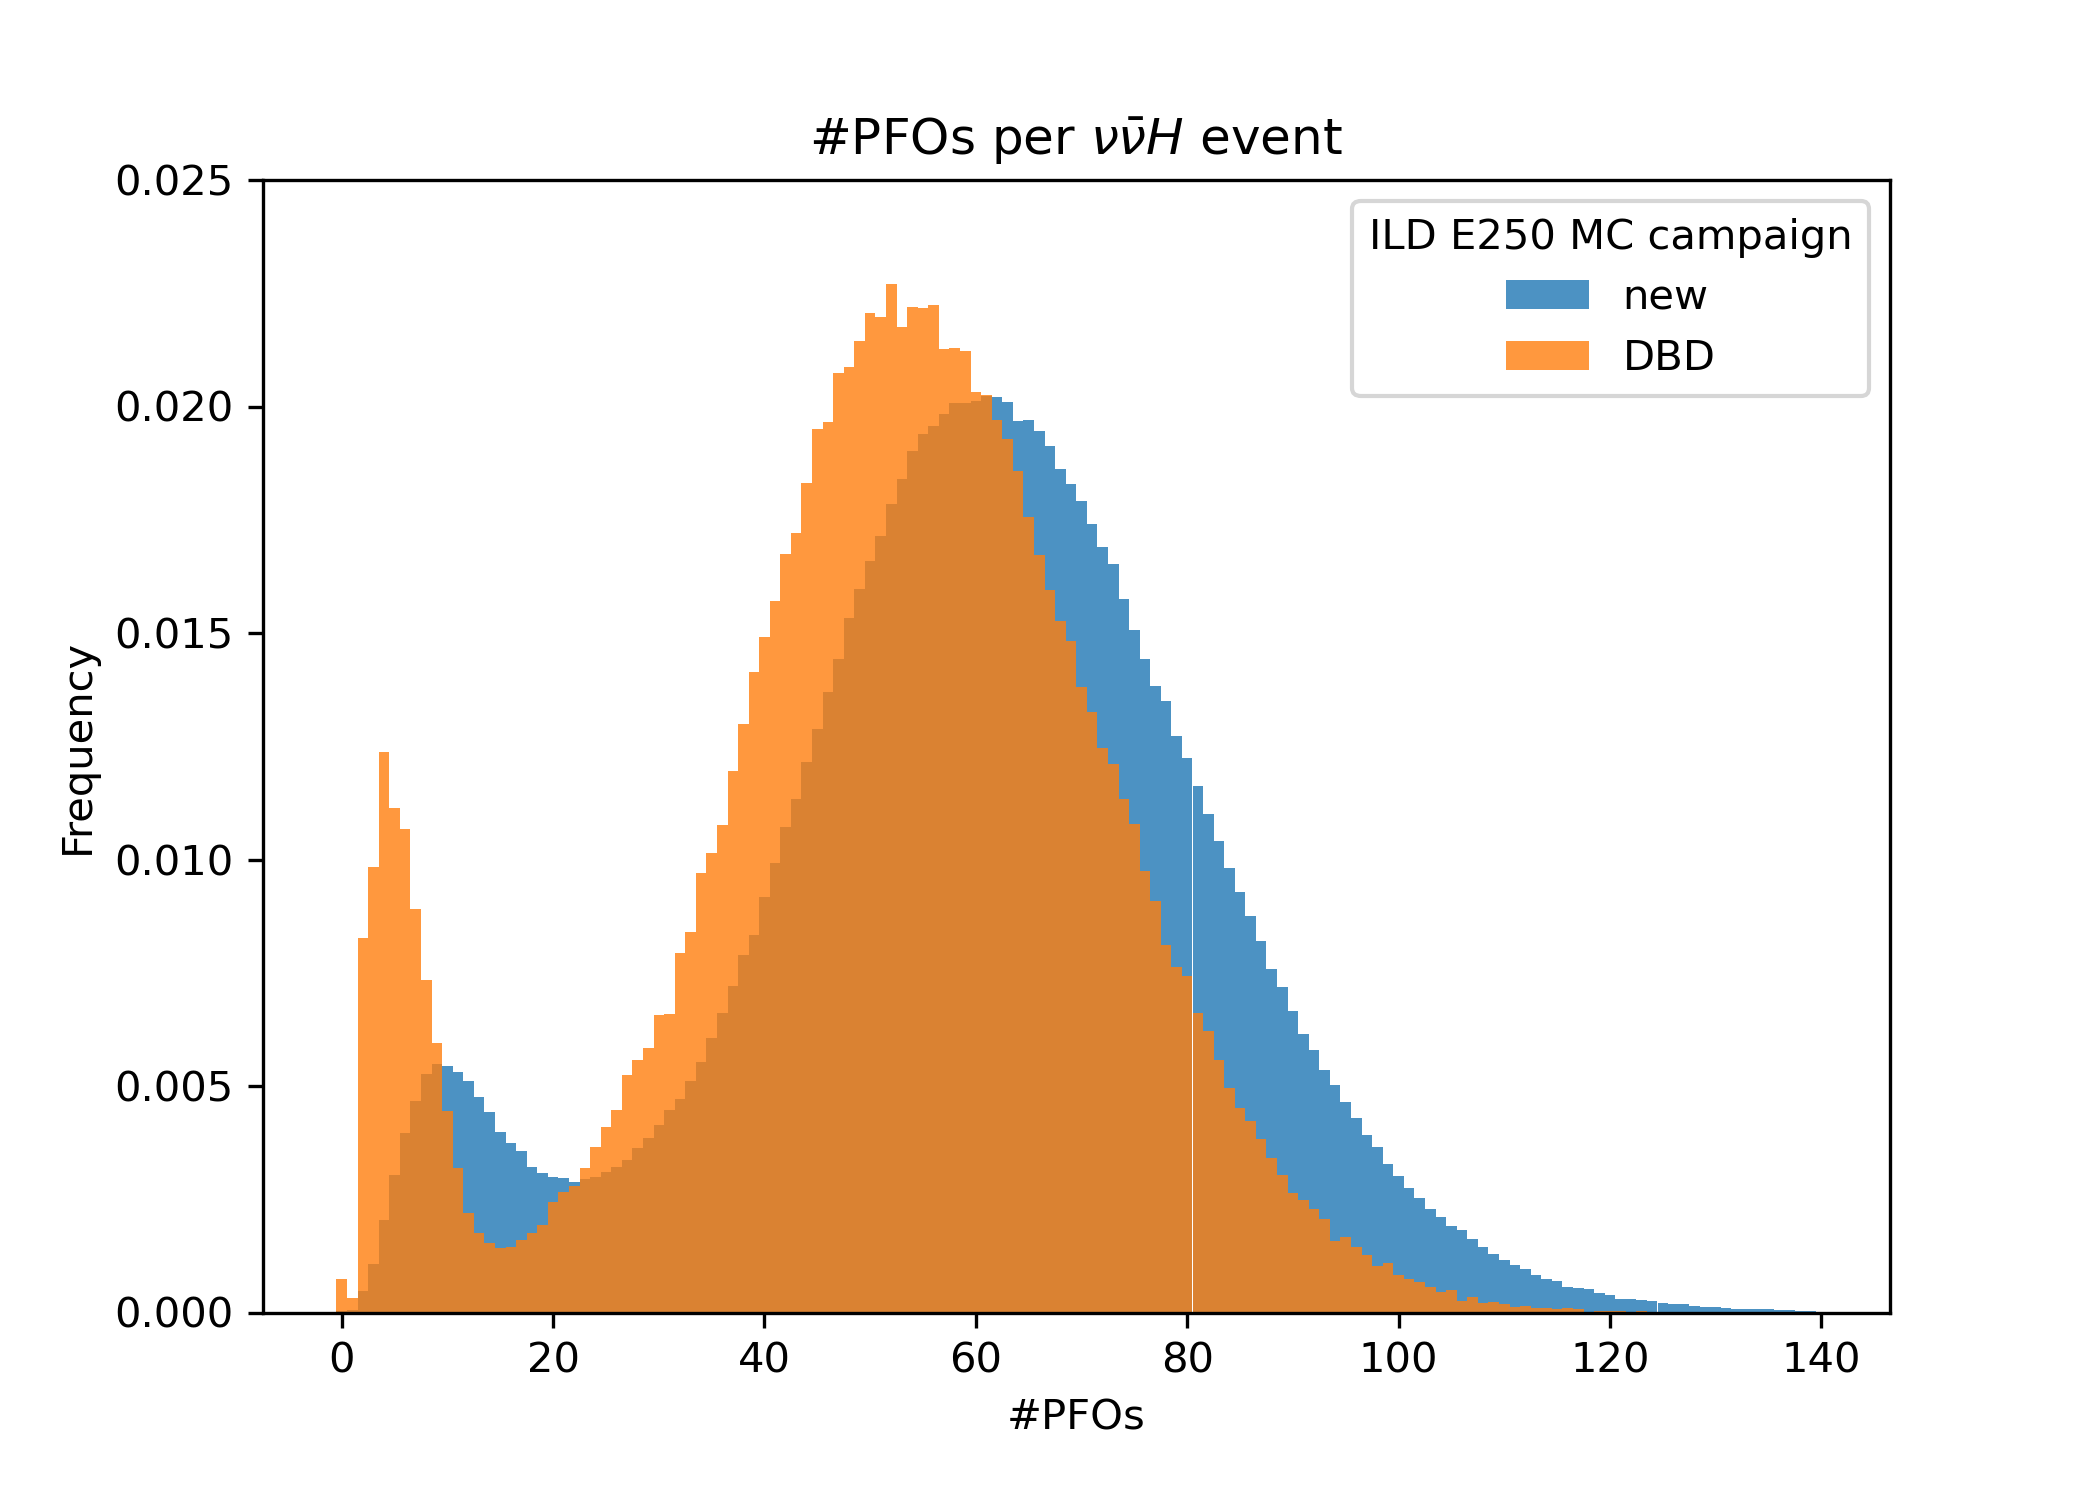
\includegraphics[height=\textheight, width=\textwidth, keepaspectratio]
        {n_pfos_full_event}};
    \node (img2) at (img1) {\only<2->{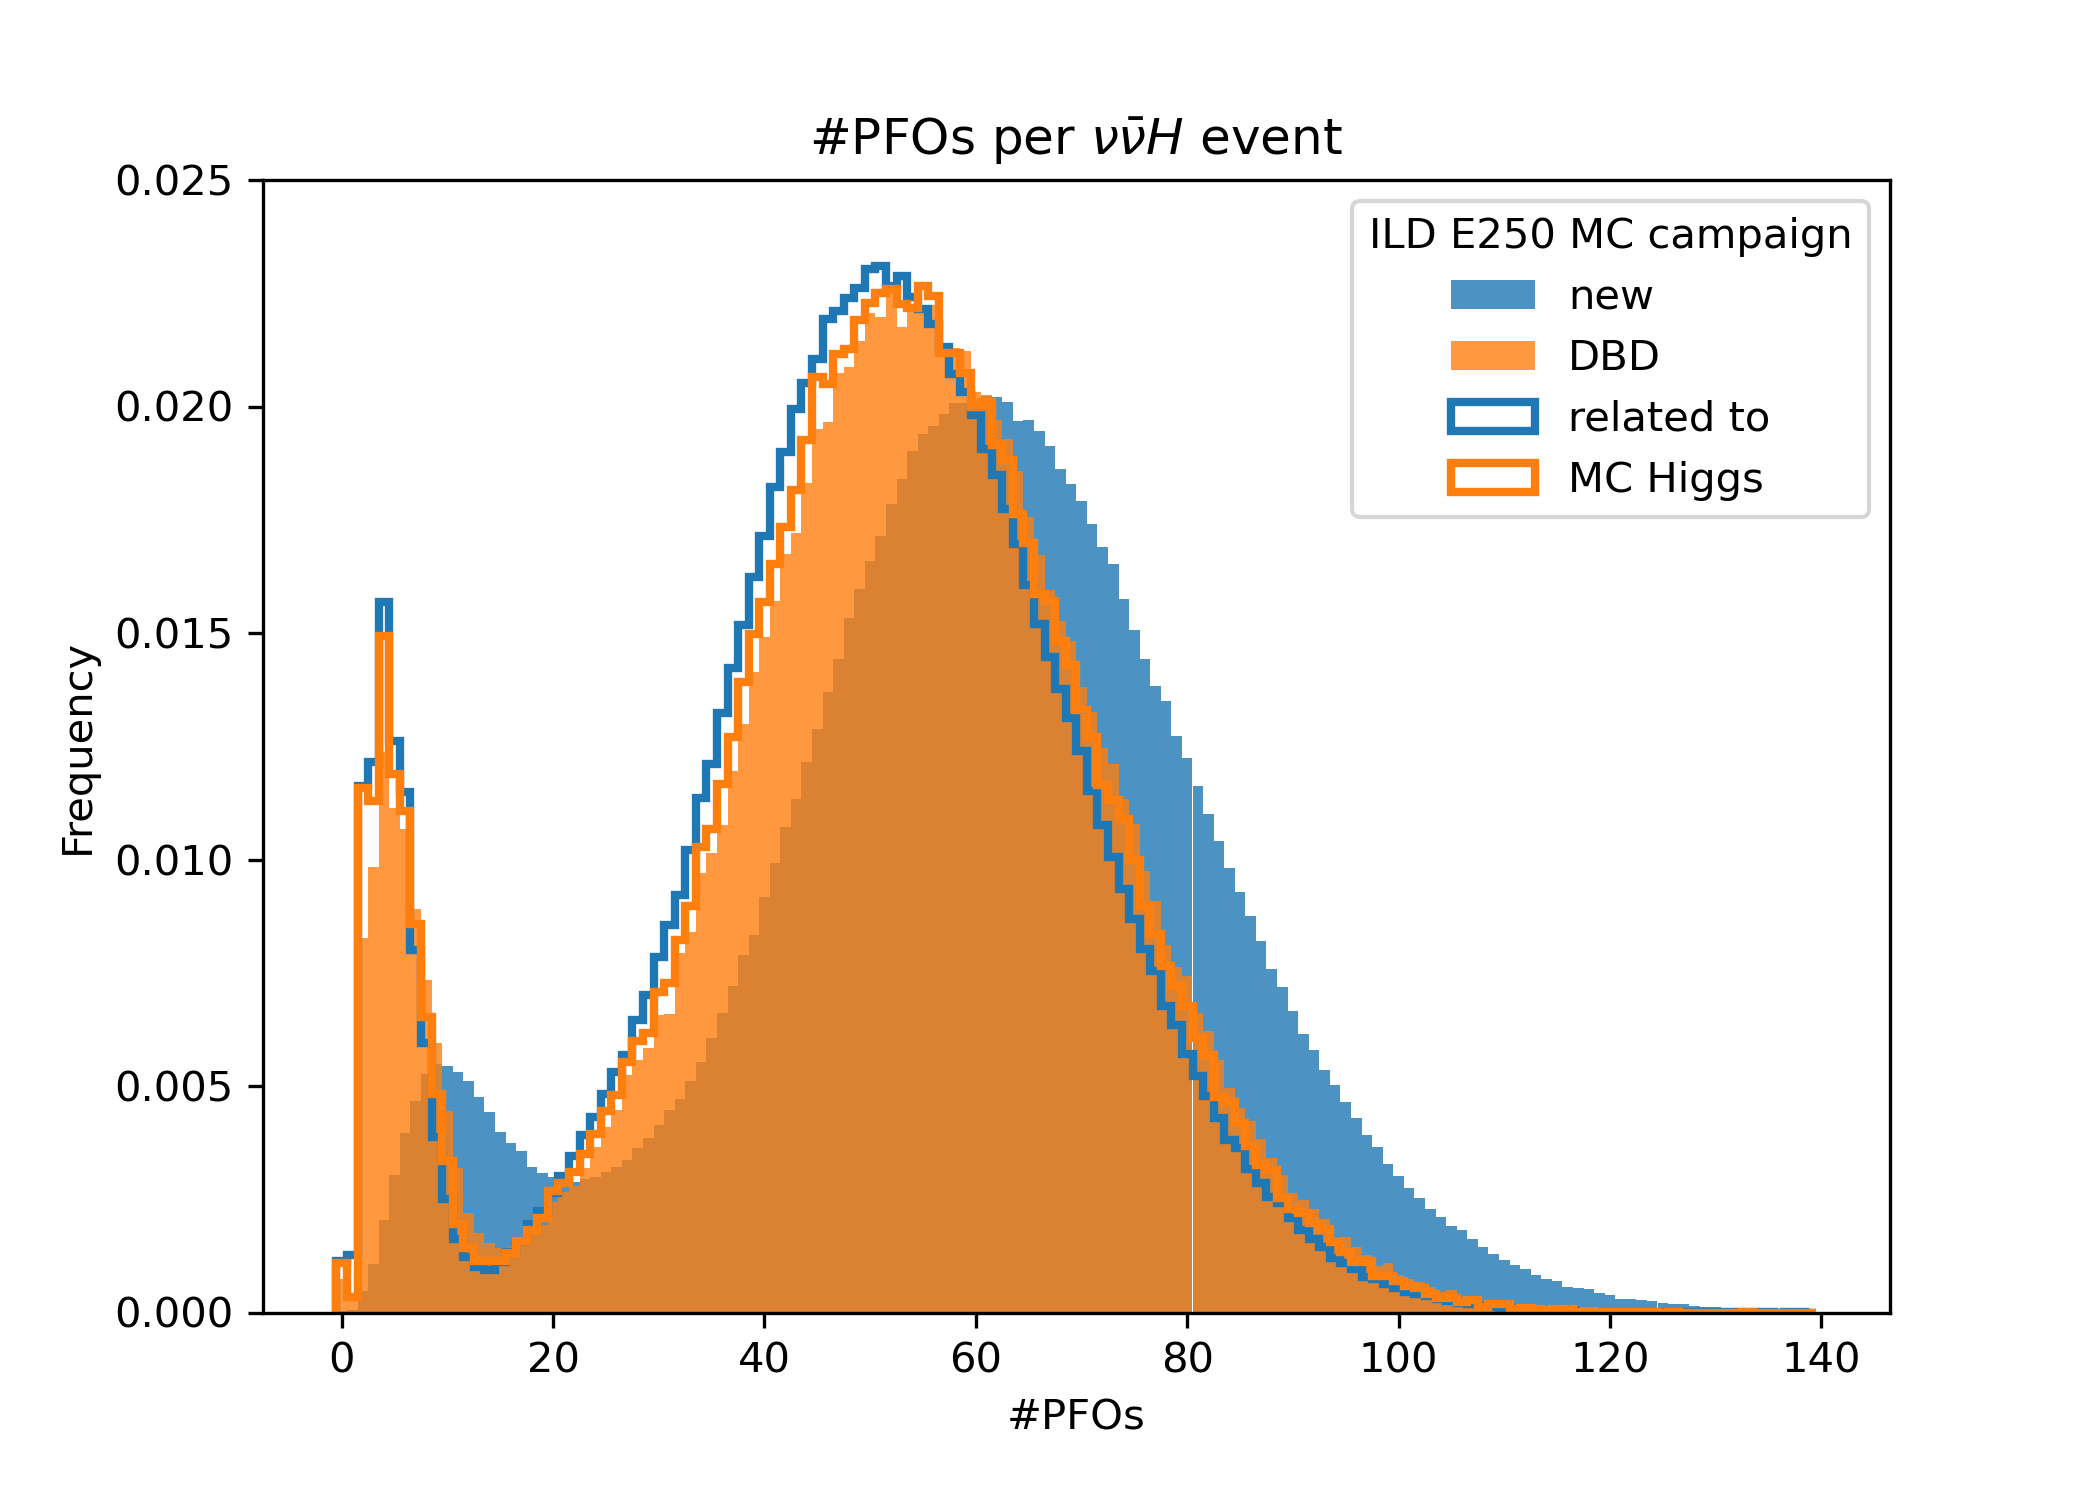
\includegraphics[height=\textheight, width=\textwidth, keepaspectratio]
        {n_pfos_full_and_only_higgs}}};
  \end{tikzpicture}
  \end{column}
  \end{columns}
  \end{frame}

\begin{frame}
  \frametitle{\textit{Global} variables}
  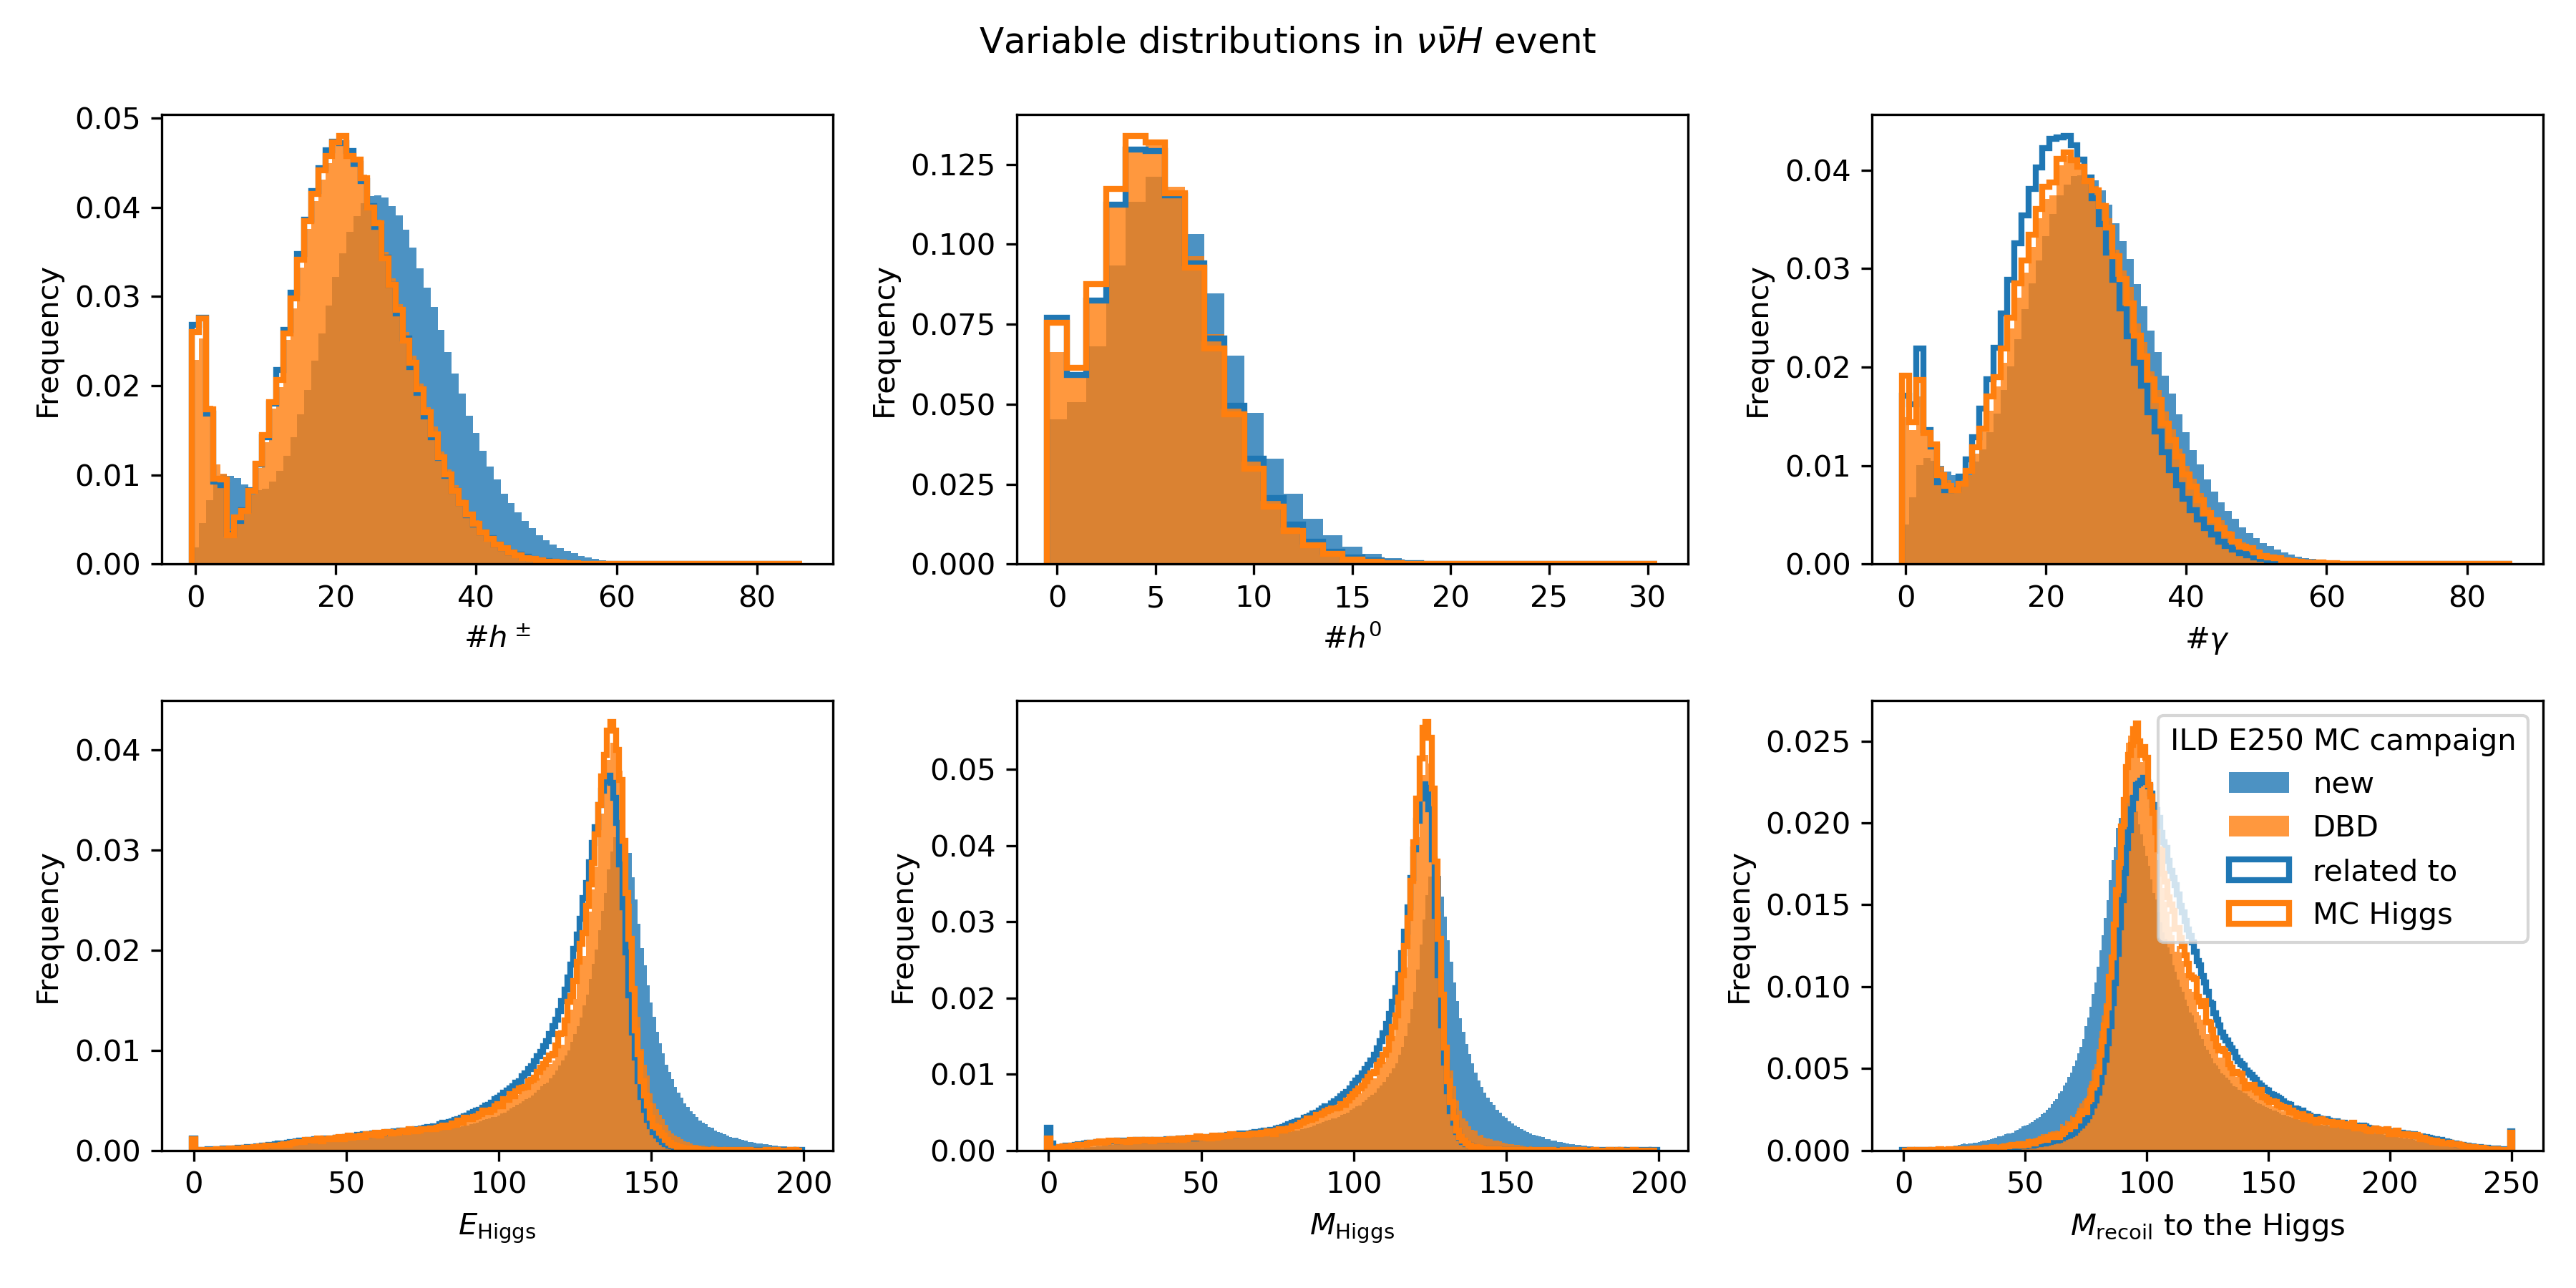
\includegraphics[height=0.9\textheight, width=\textwidth, keepaspectratio]
      {many_variables_full_and_only_higgs}
  \end{frame}

\begin{frame}
  \frametitle{Overlay composition}
  Frequency and size of the overlay increased, composition altered.
  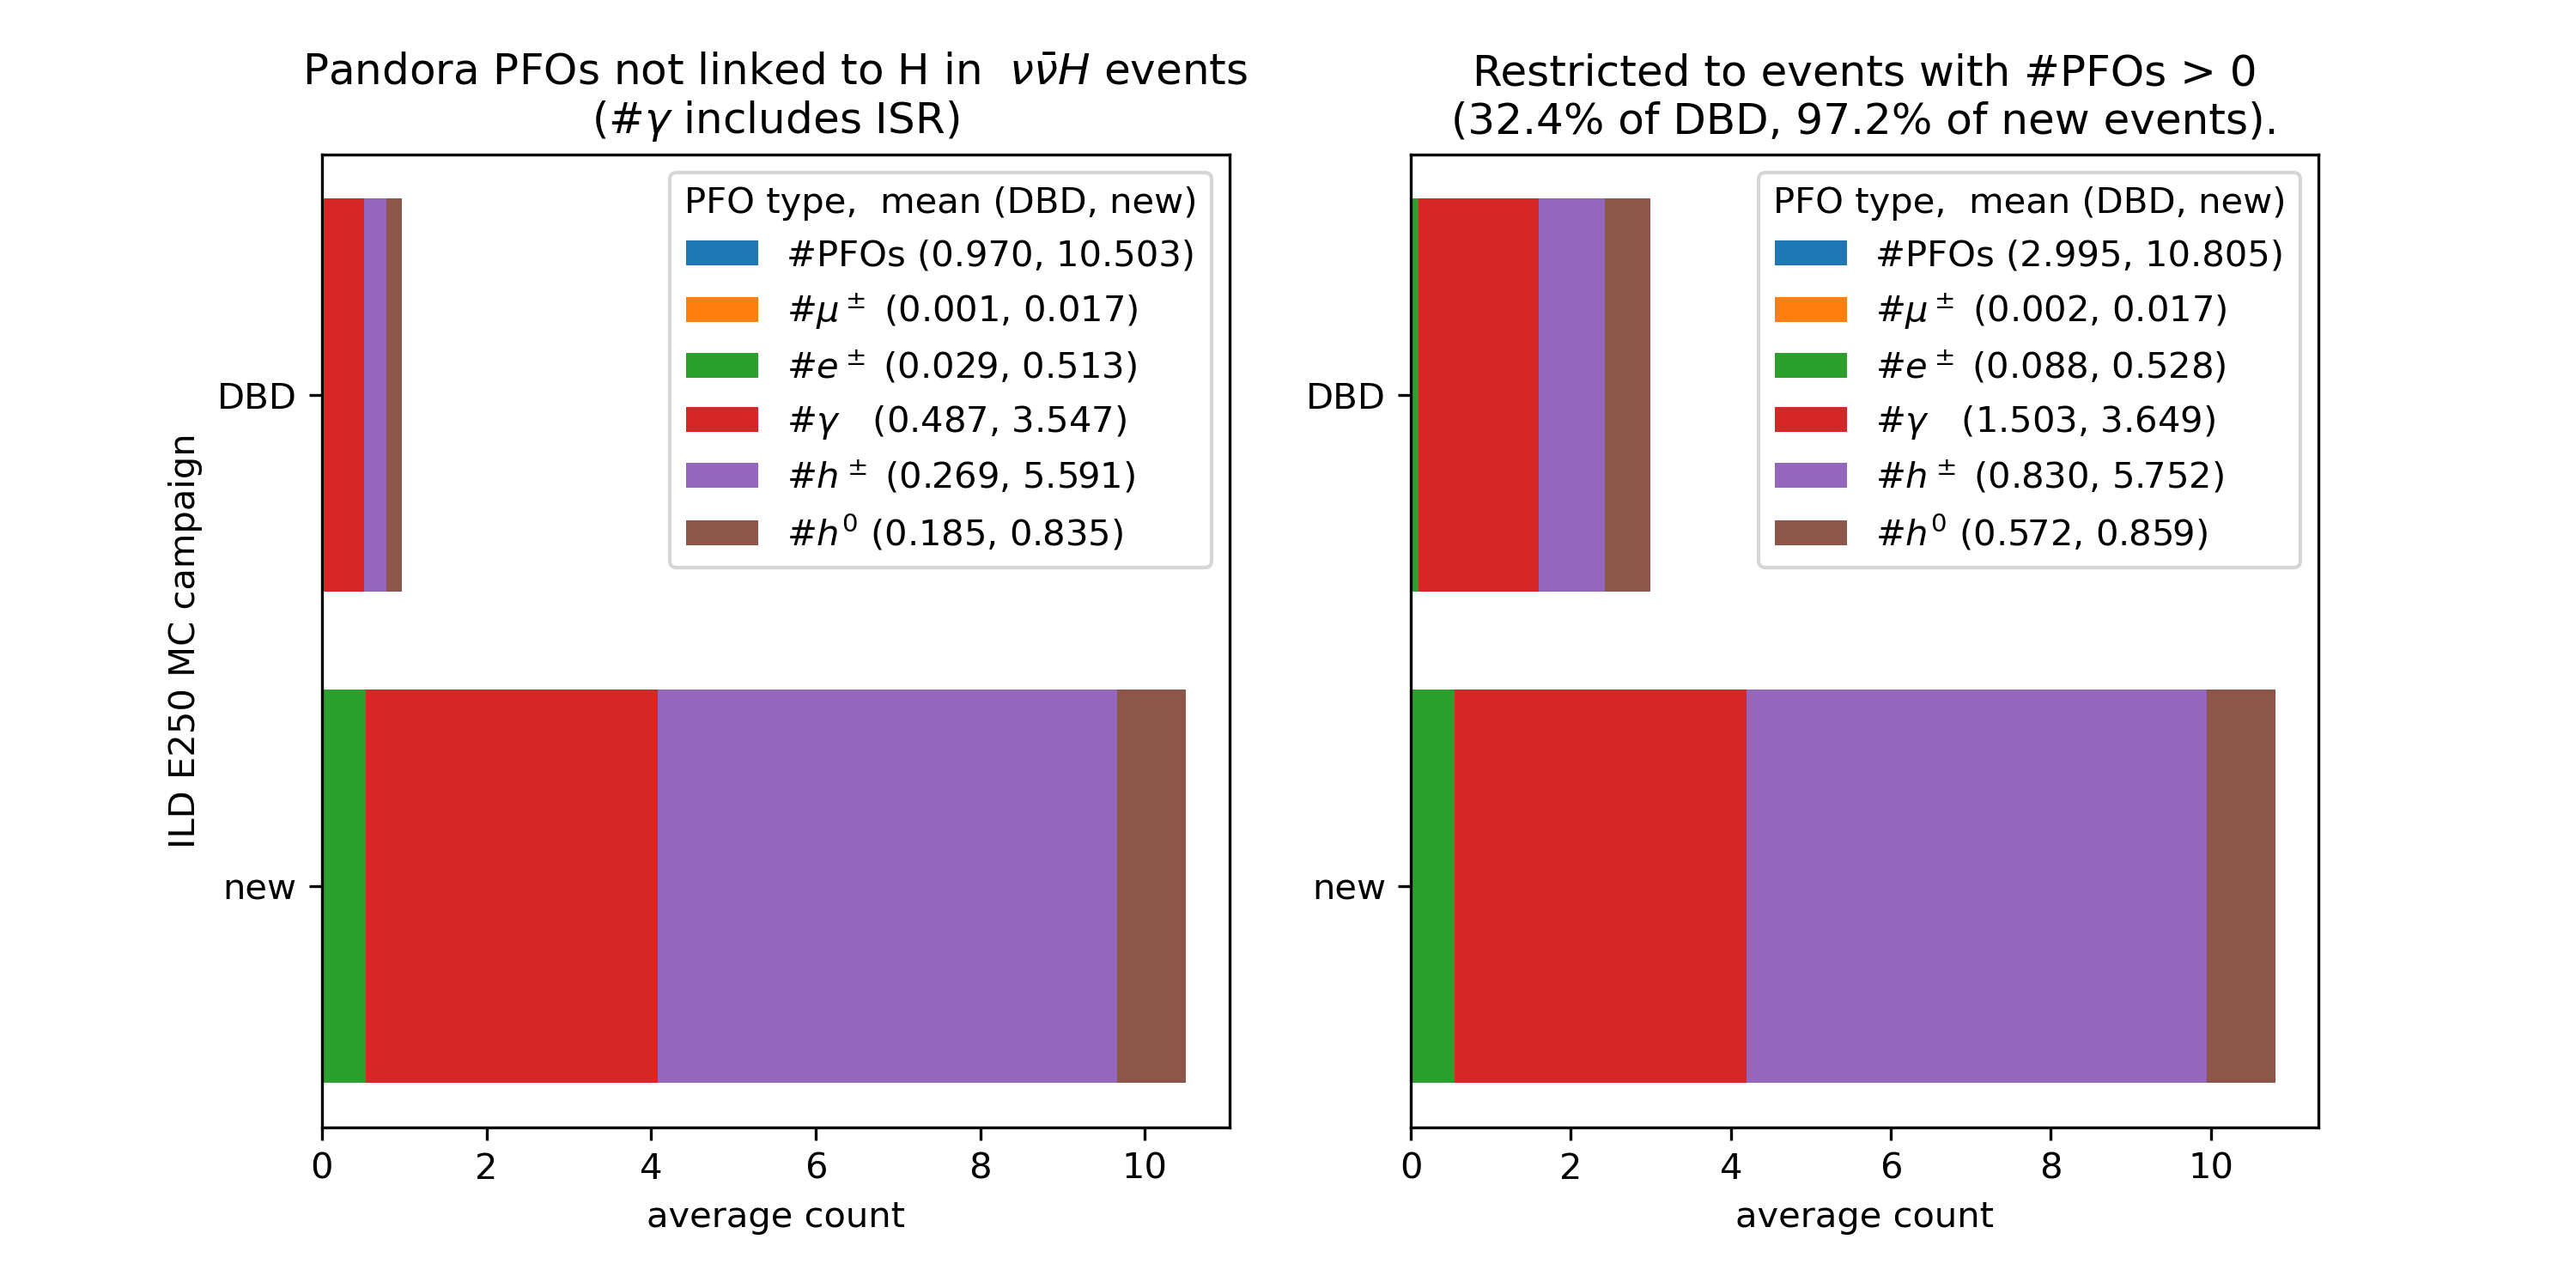
\includegraphics[height=0.8\textheight, width=\textwidth, keepaspectratio]
      {overlay_counts_per_group}
  \end{frame}

\begin{frame}
  \frametitle{Overlay shape}
  Frequency and size of the overlay increased, composition altered.
  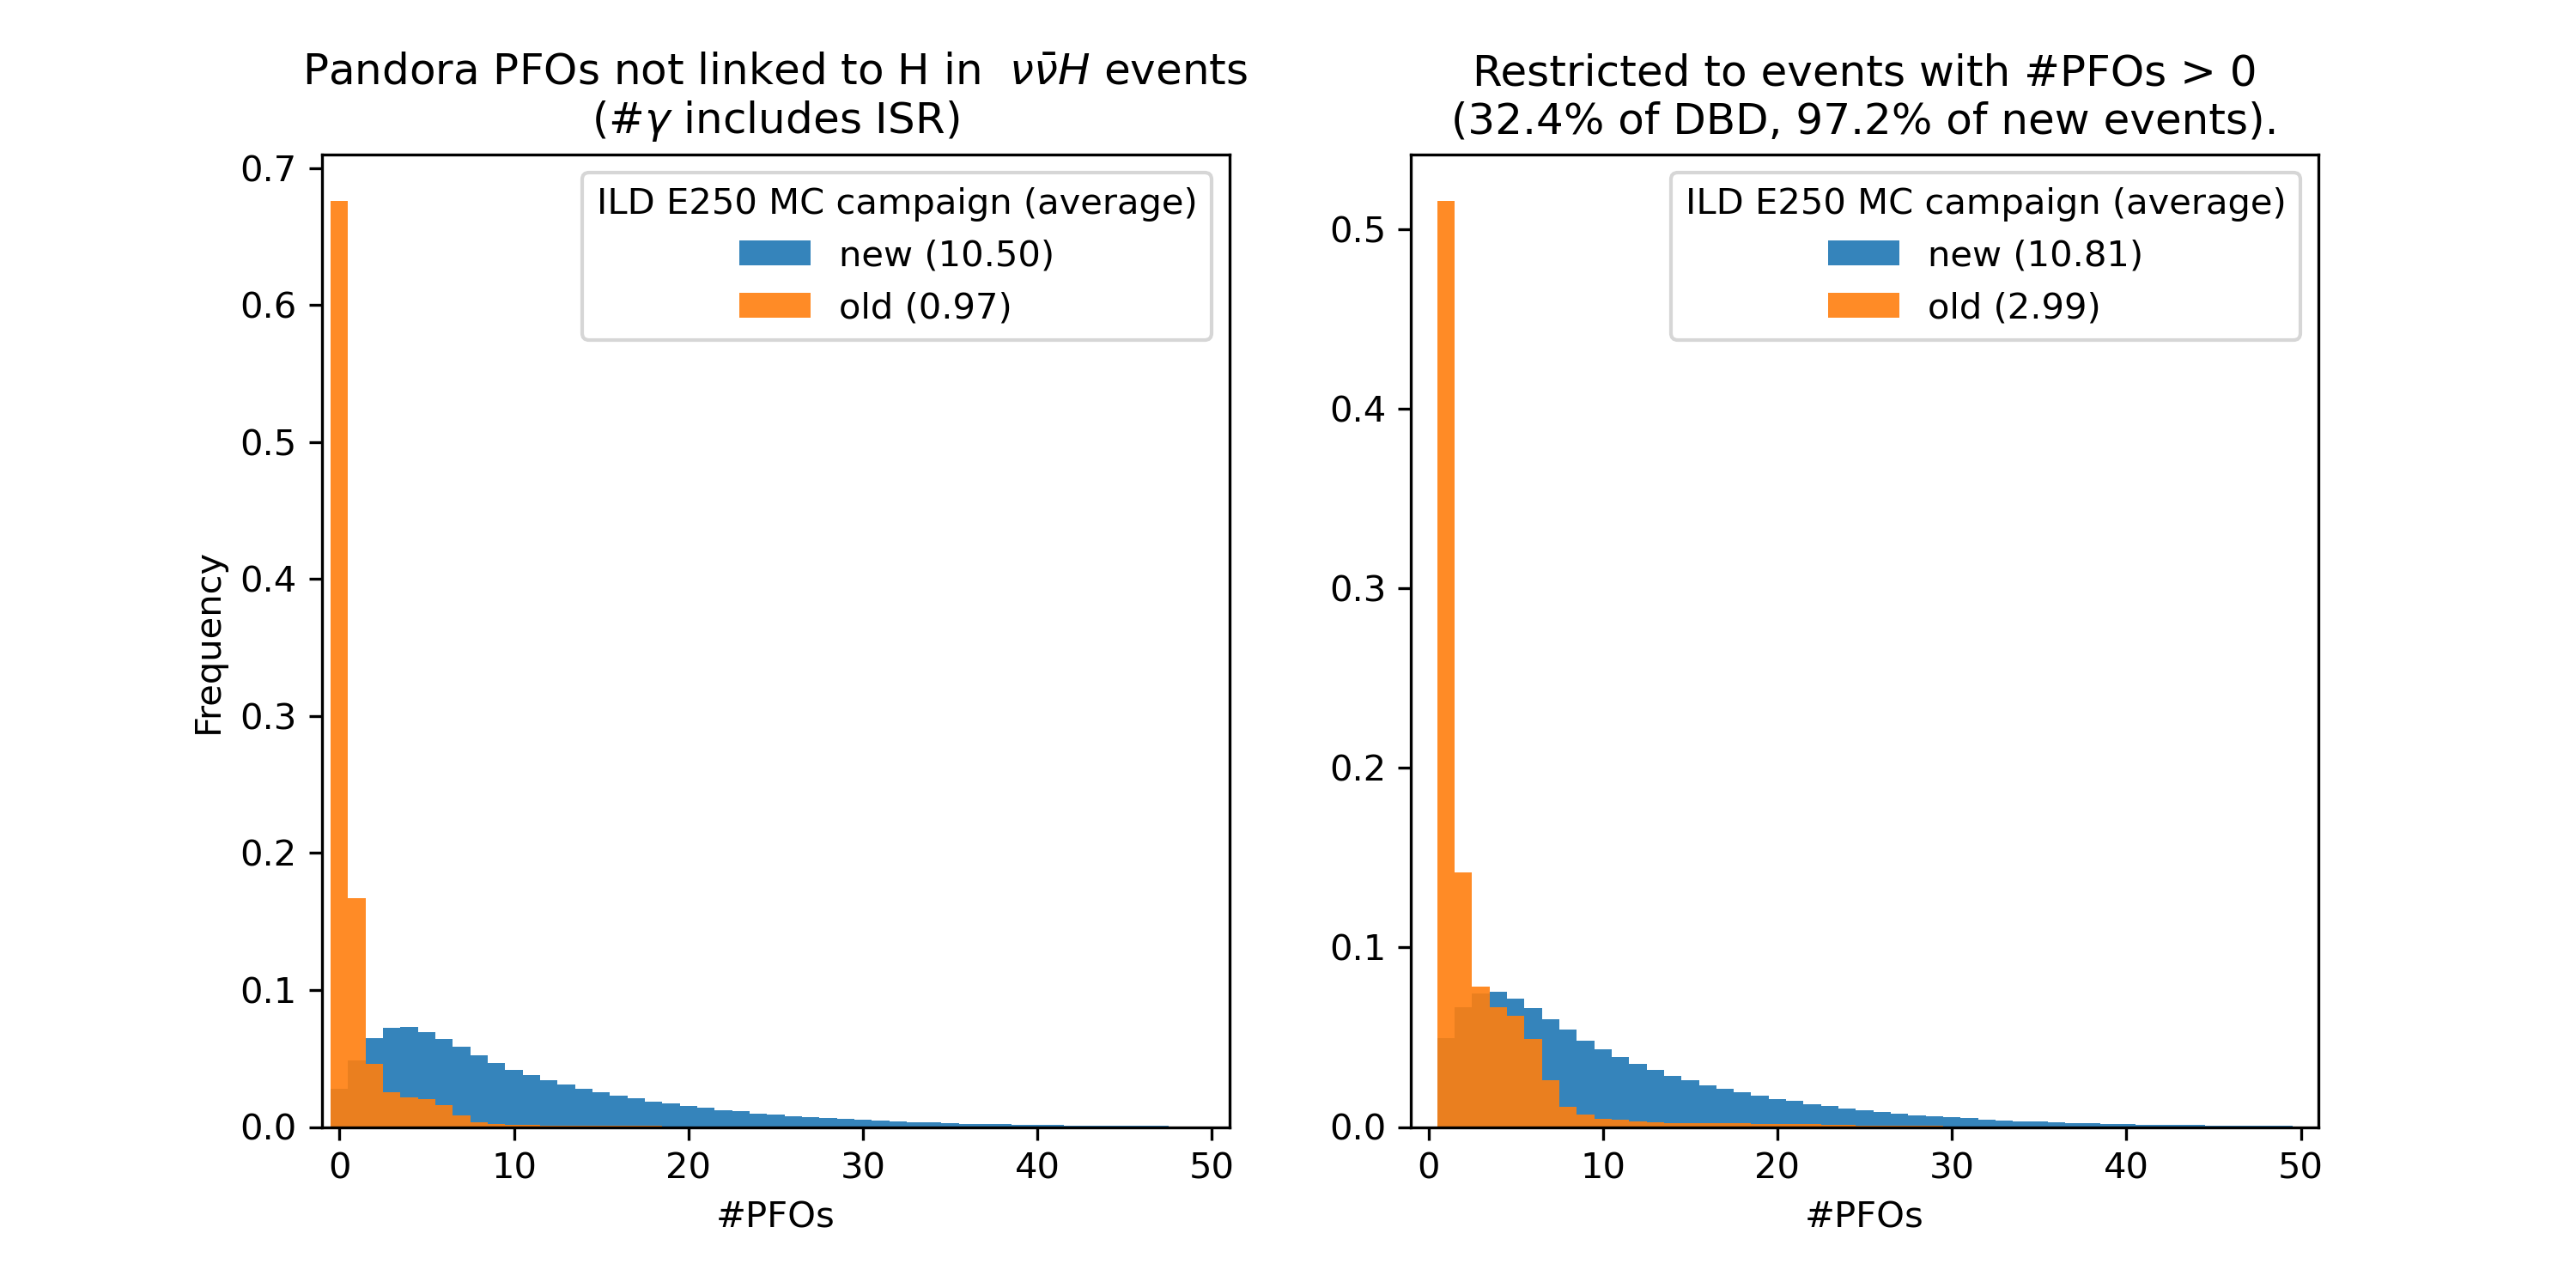
\includegraphics[height=0.8\textheight, width=\textwidth, keepaspectratio]
      {overlay_n_pfos}
  \end{frame}

\begin{frame}
  \frametitle{Overlay shape - log scale}
  Frequency and size of the overlay increased, composition altered.
  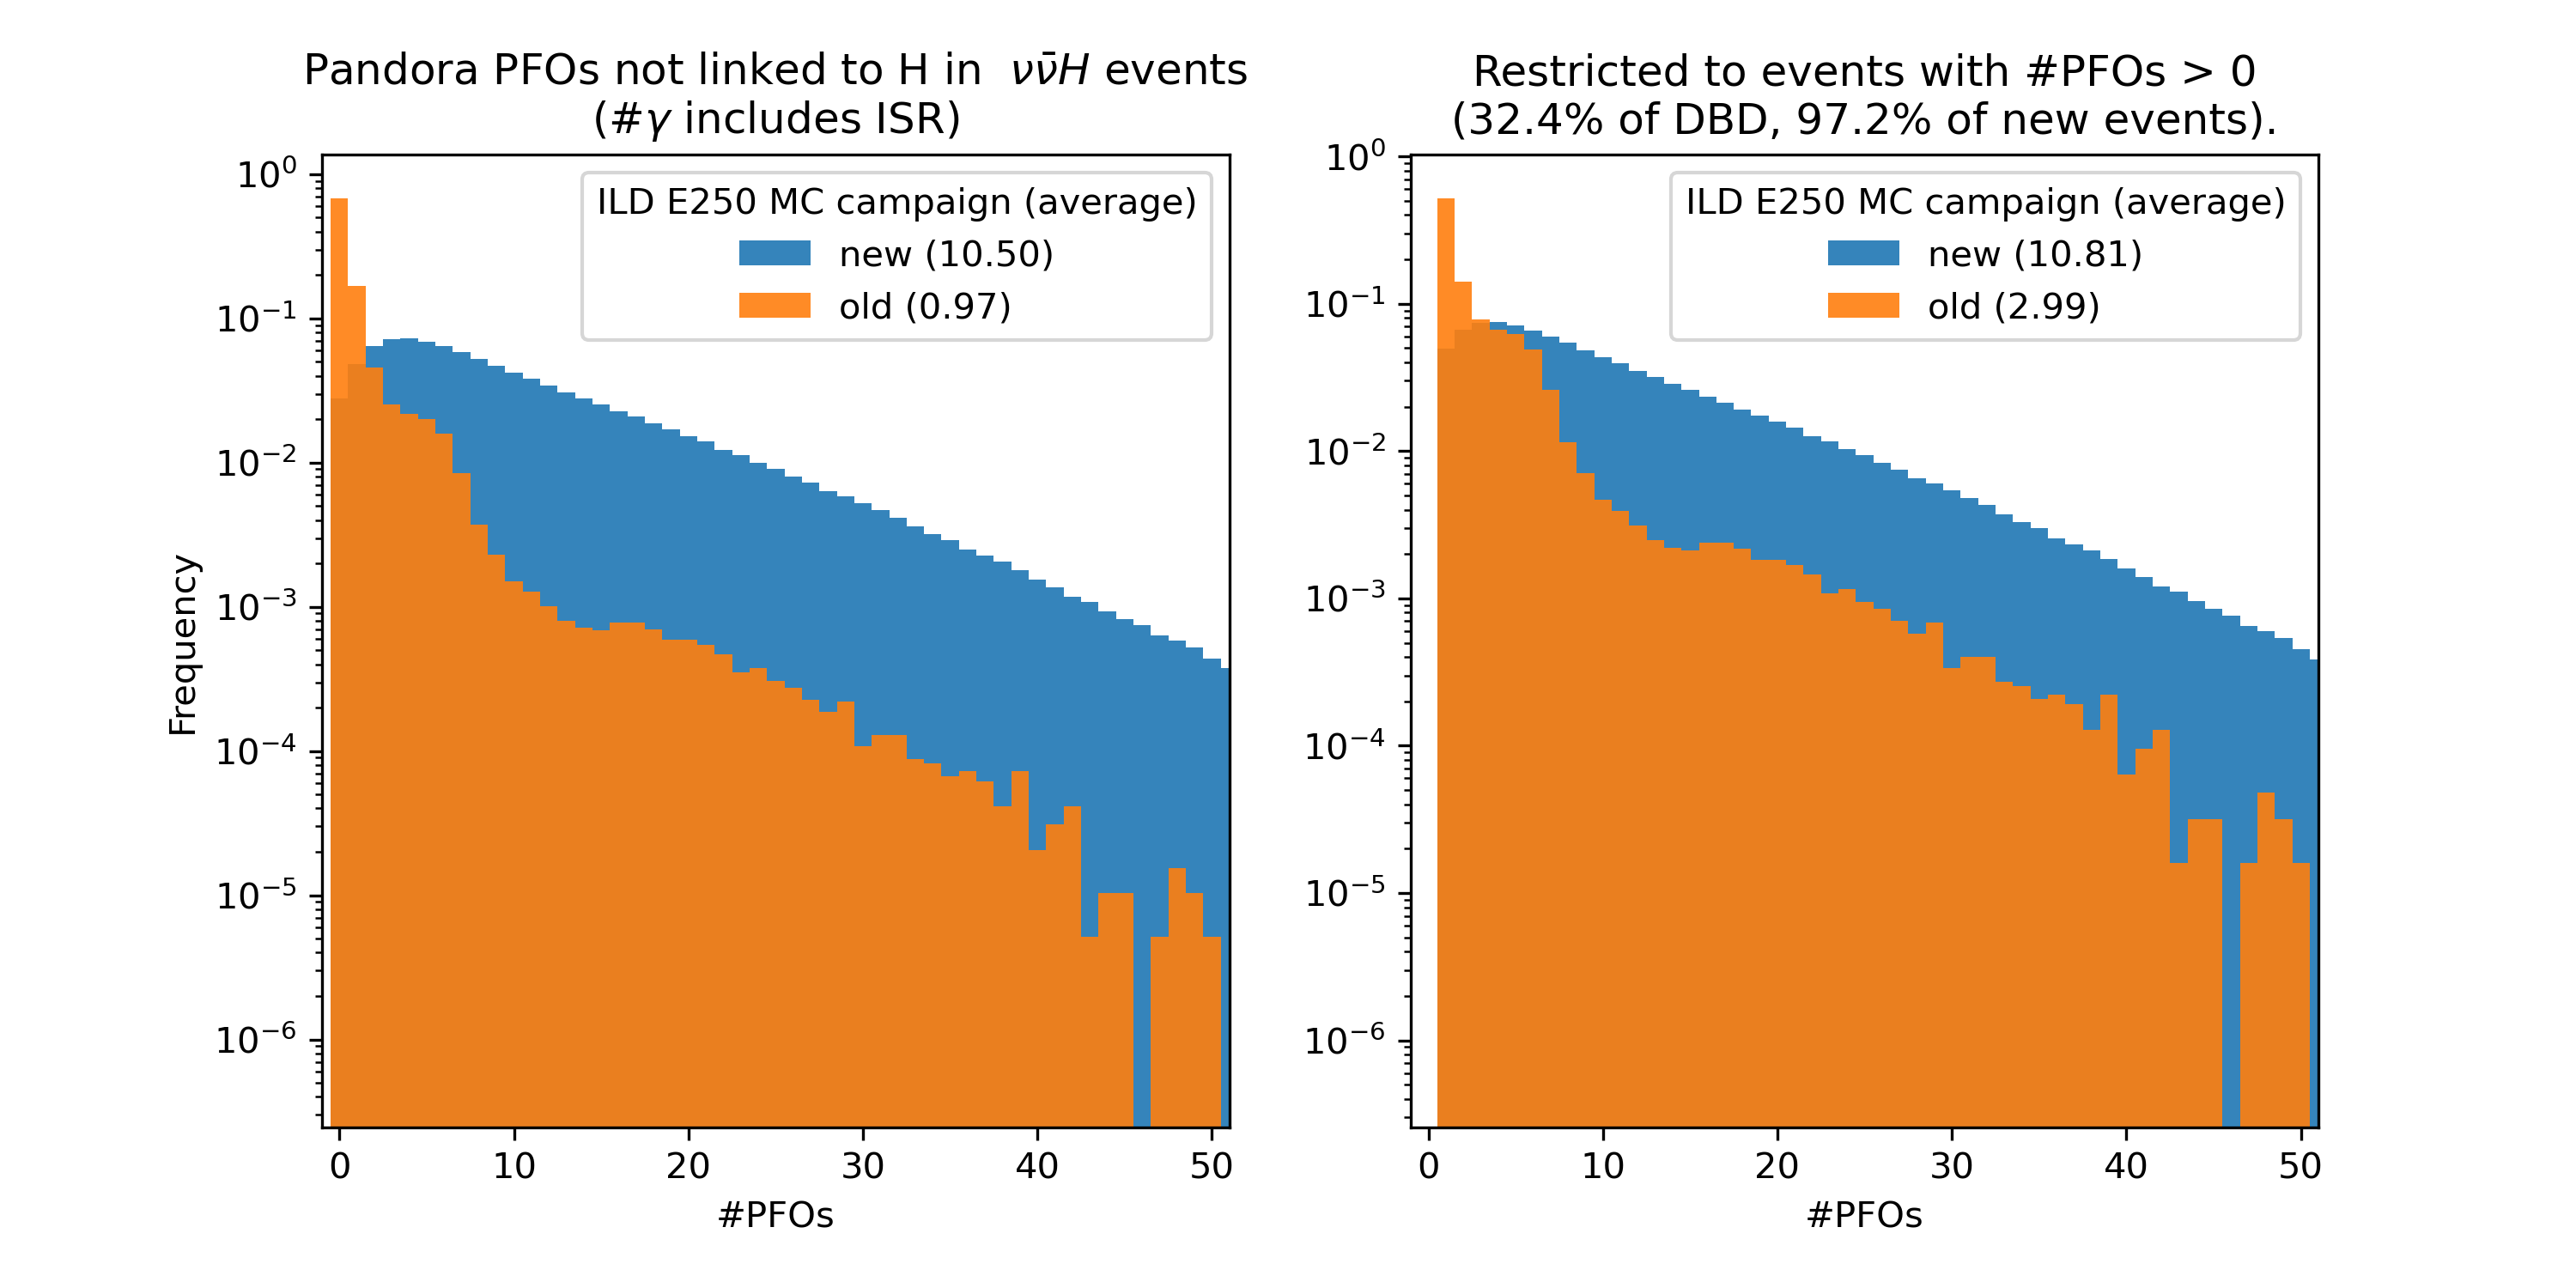
\includegraphics[height=0.8\textheight, width=\textwidth, keepaspectratio]
      {overlay_n_pfos_log}
  \end{frame}

\begin{frame}
  \frametitle{Overlay energy}
  On average $\approx10~\GeV$. $E_{\tn{Higgs}}^{\tn{mean}}\approx130~\GeV$.
  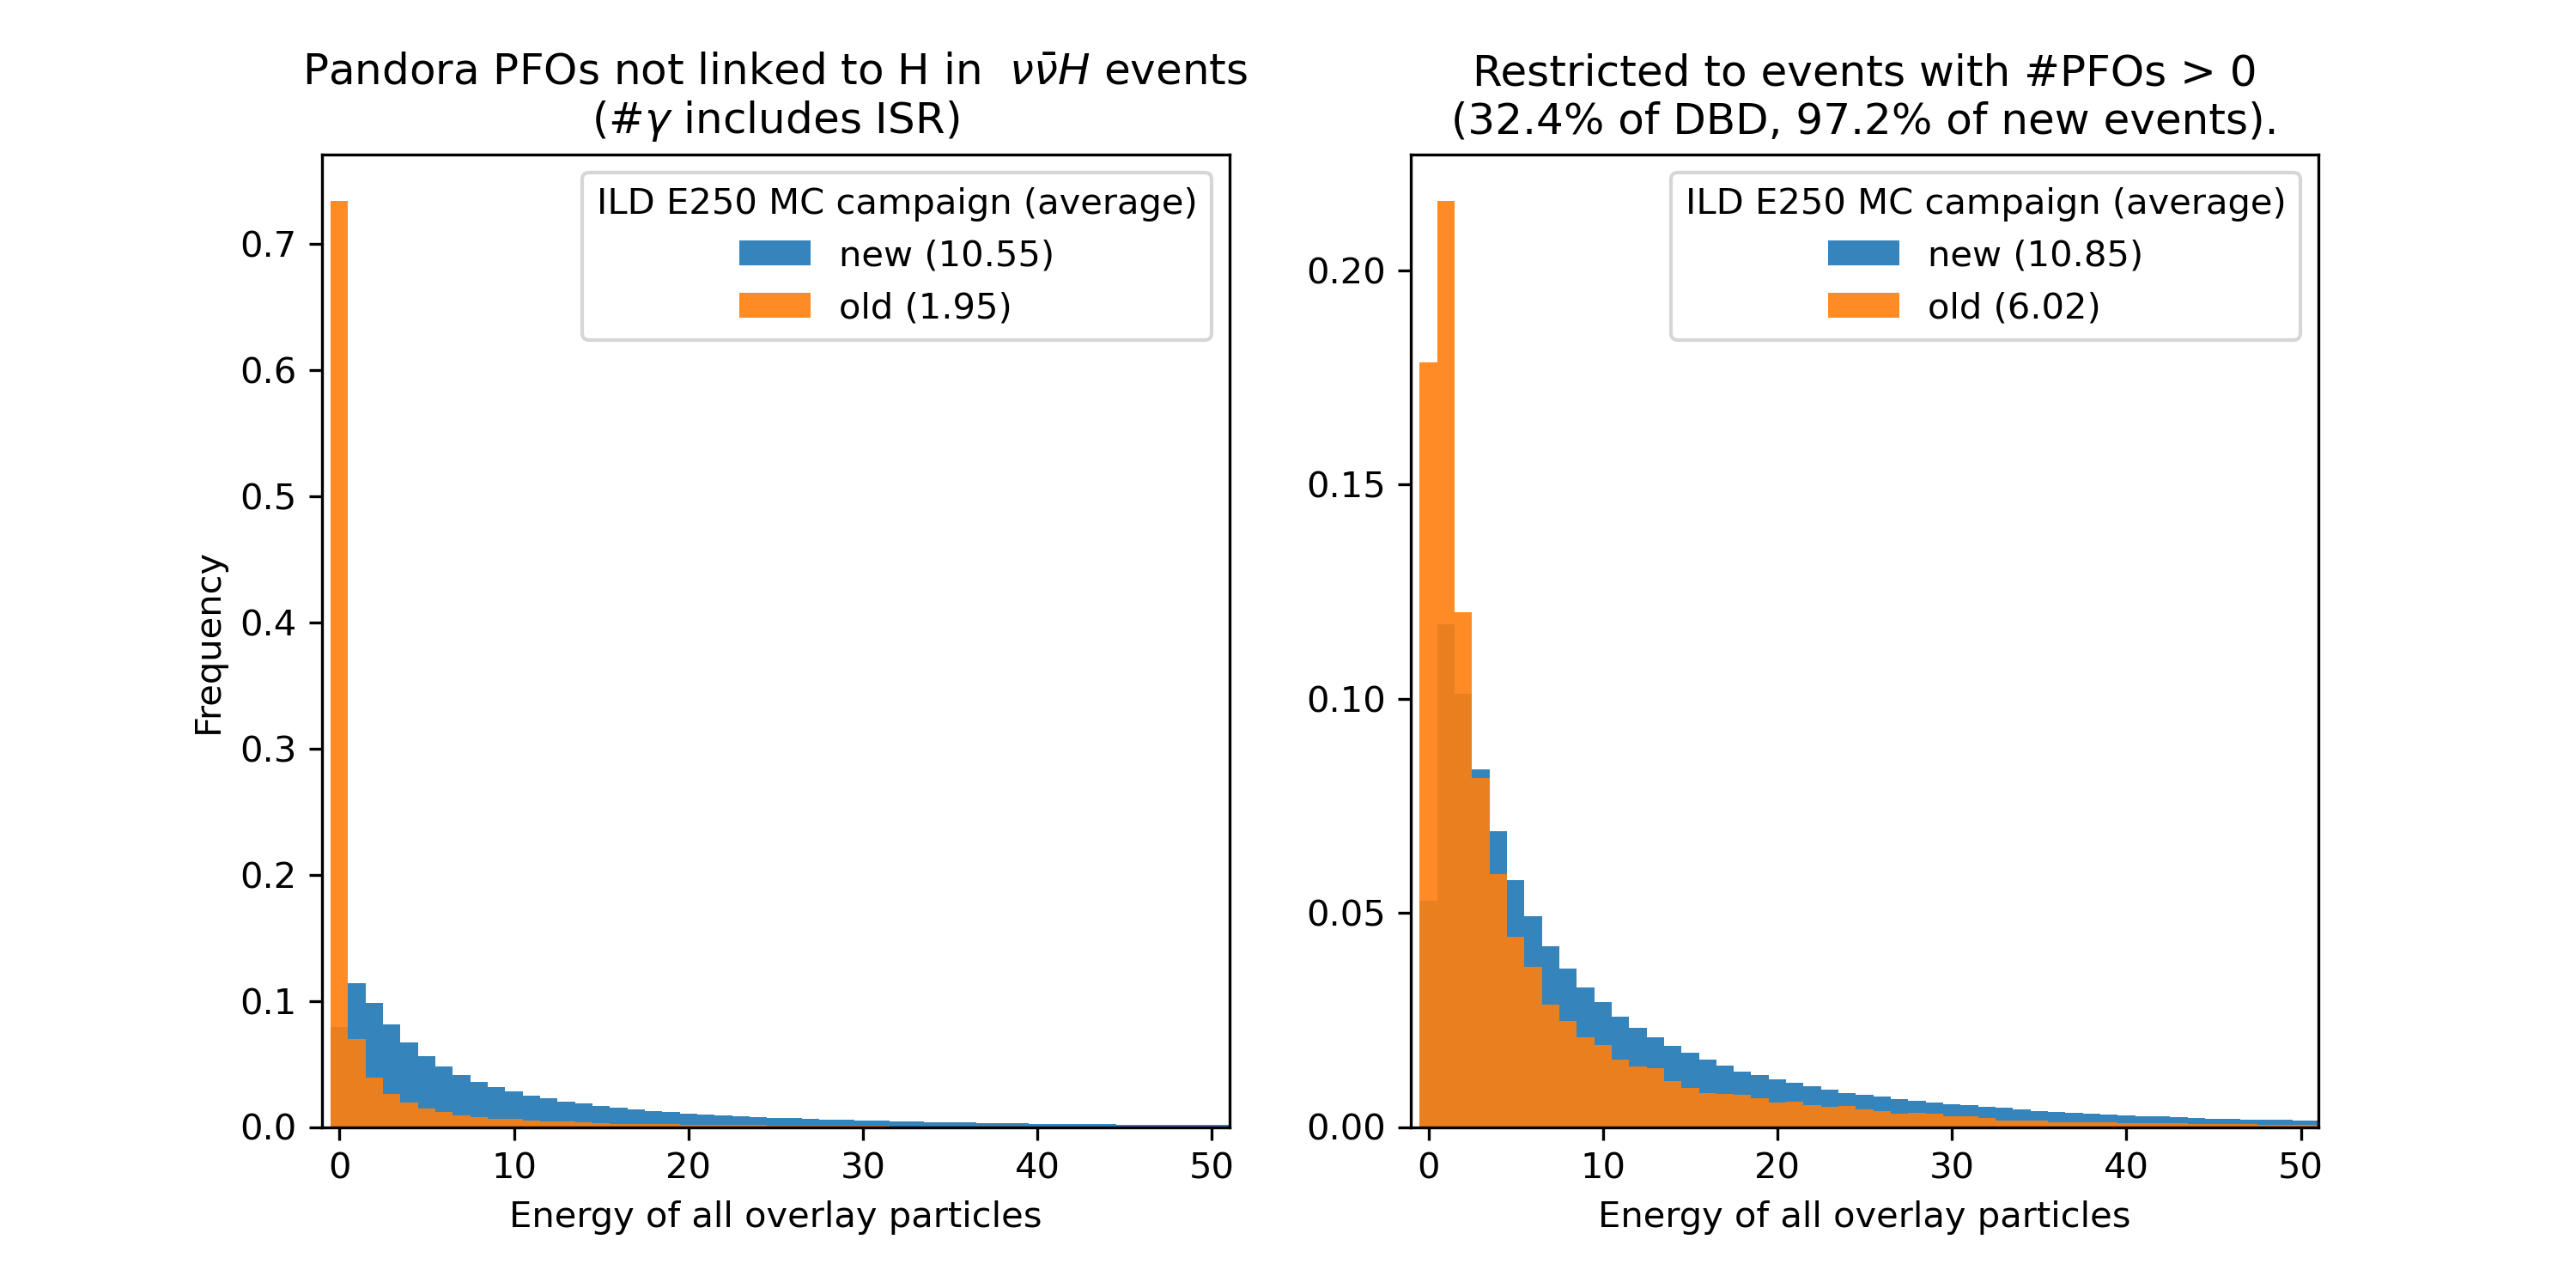
\includegraphics[height=0.8\textheight, width=\textwidth, keepaspectratio]
      {overlay_energy}
  \end{frame}

\begin{frame}
  \frametitle{Overlay energy}
  On average $\approx10~\GeV$. $E_{\tn{Higgs}}^{\tn{mean}}\approx130~\GeV$.
  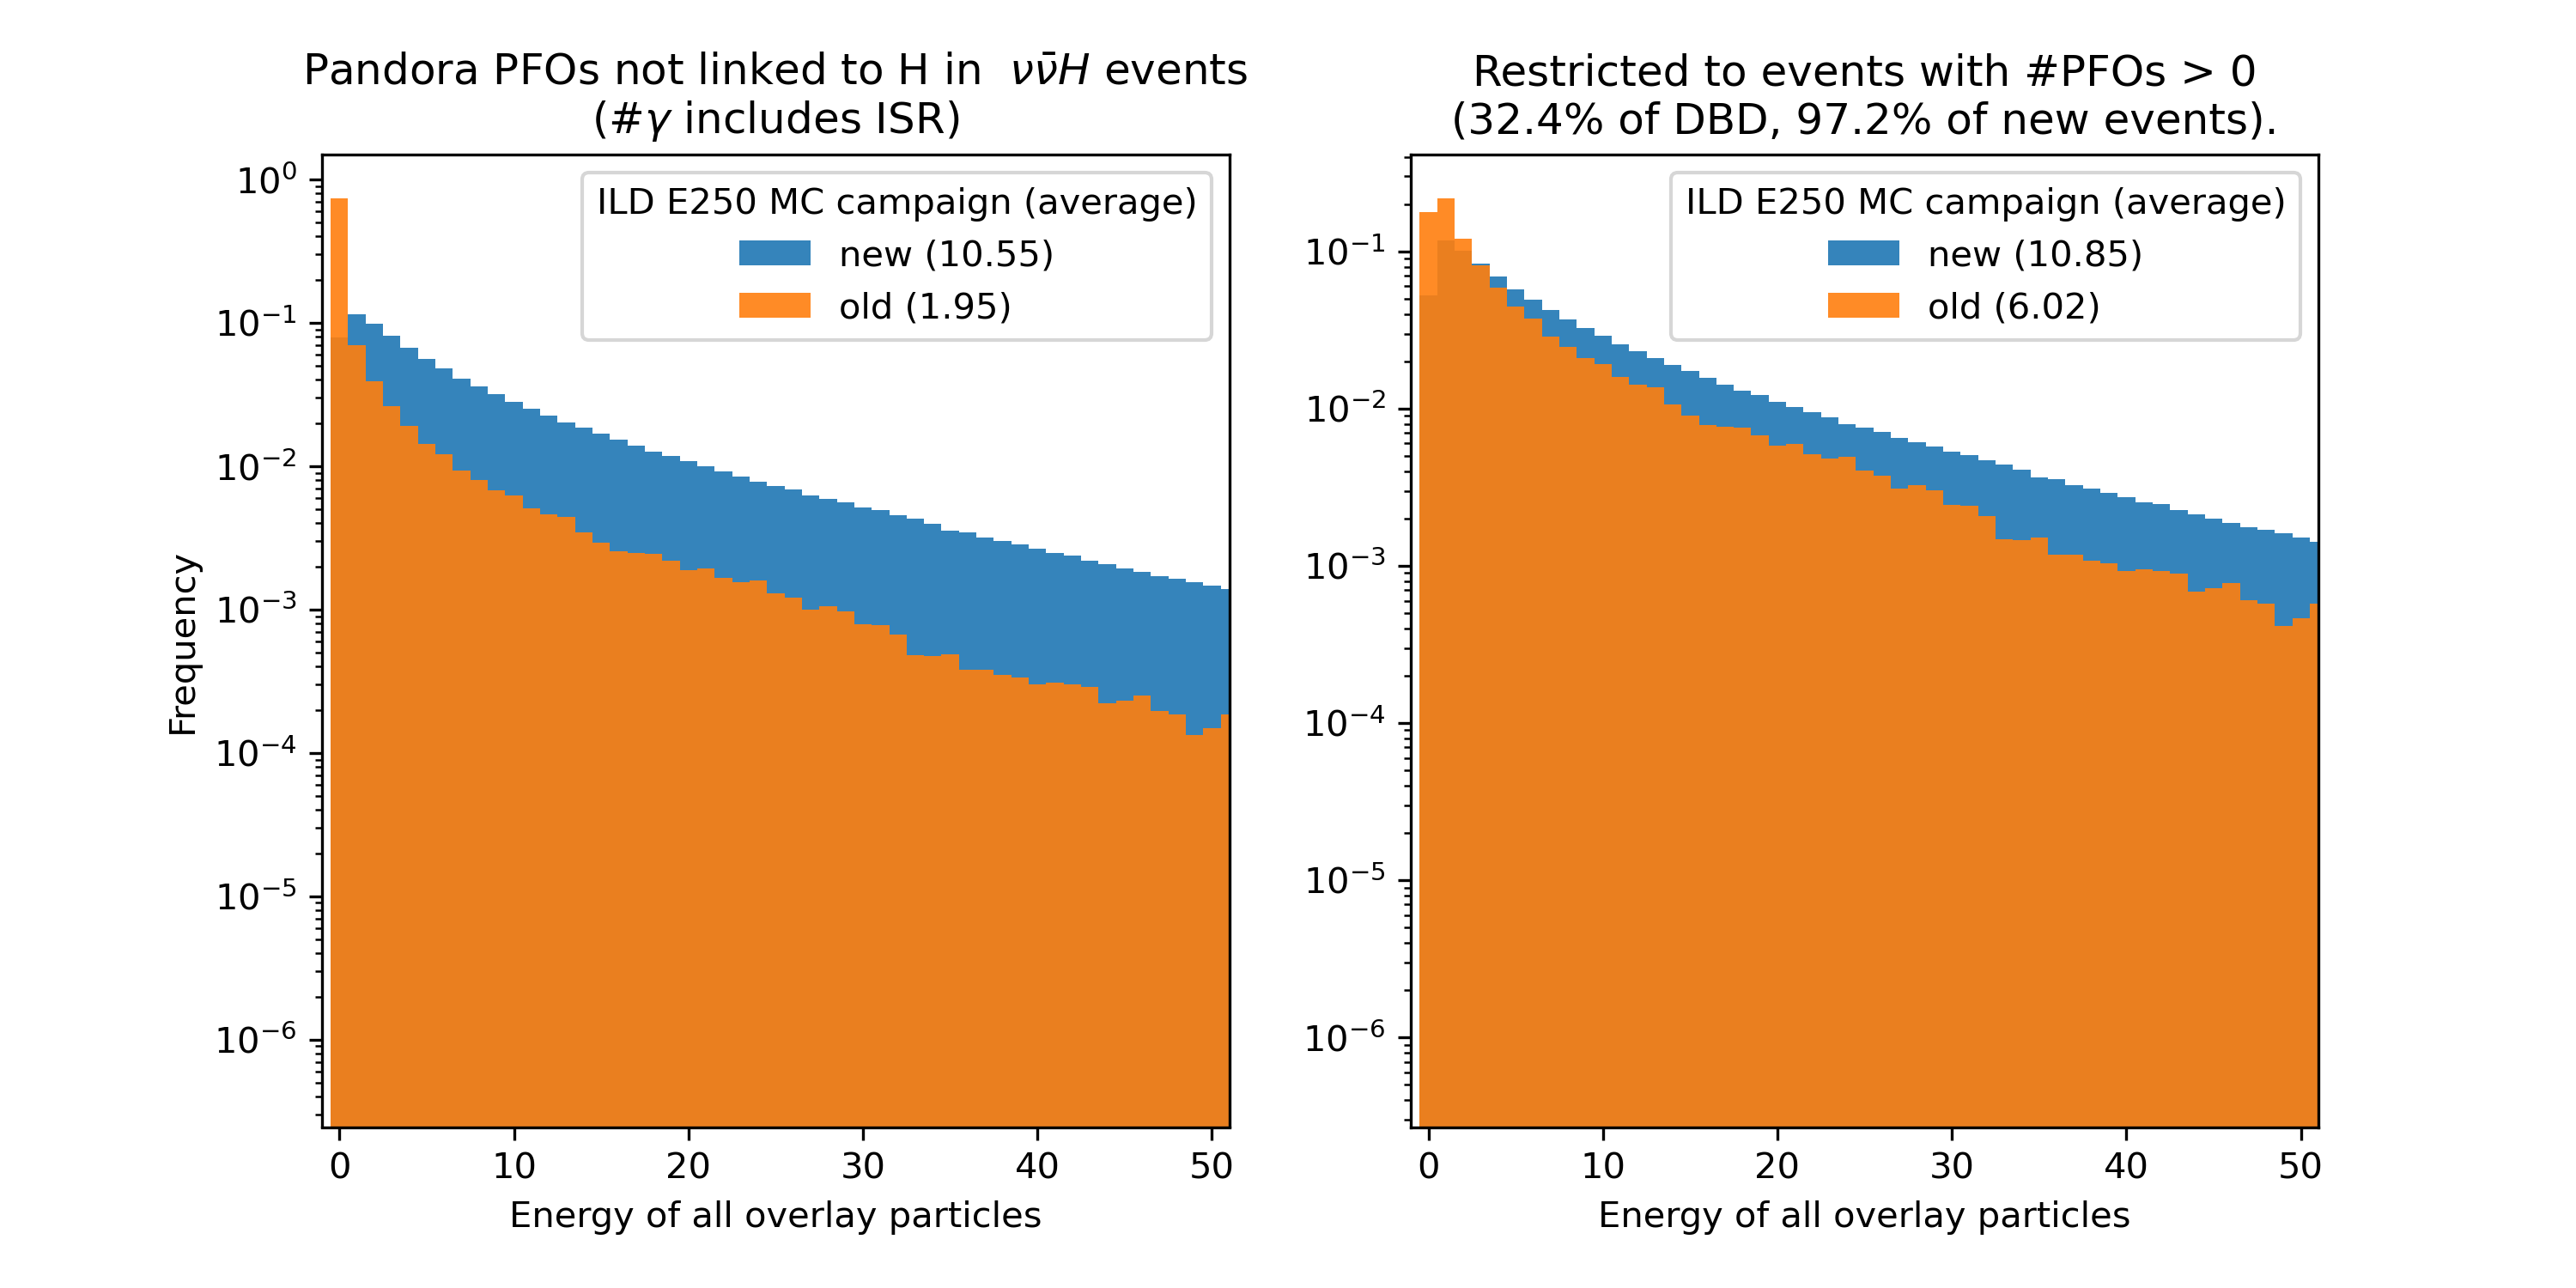
\includegraphics[height=0.8\textheight, width=\textwidth, keepaspectratio]
      {overlay_energy_log}
  \end{frame}

\begin{frame}
  \frametitle{Isolated Leptons}
  Using the IsolatedLeptonTaggingProcessor with DBD weights.
  \begin{center}
    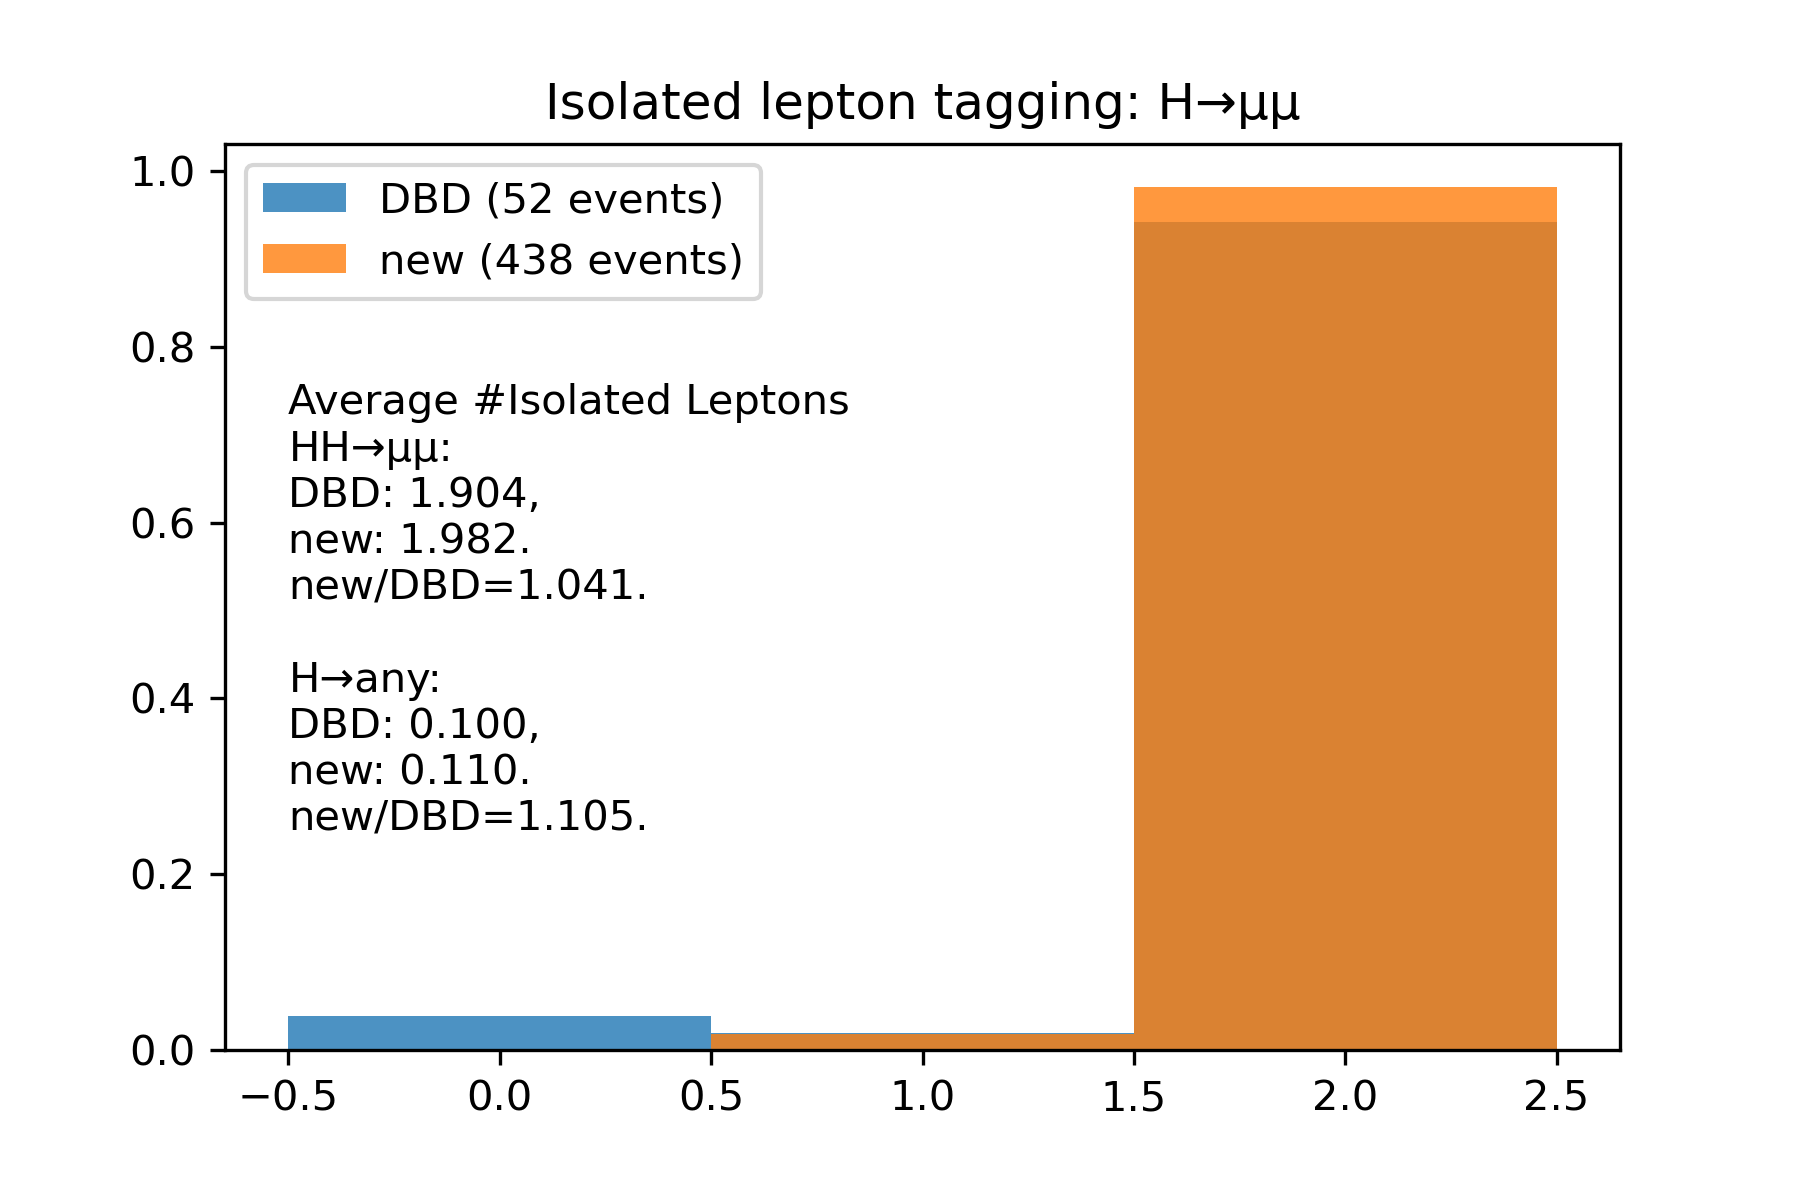
\includegraphics[height=0.8\textheight, width=\textwidth, keepaspectratio]
        {isolated_leptons}
  \end{center}
  \end{frame}

\begin{frame}
  \frametitle{Branching ratios}
  \begin{columns}[c,onlytextwidth]
  \begin{column}{0.5\textwidth}
  Differences (red) seem to be larger than statistical uncertainty.
  \newline\newline
  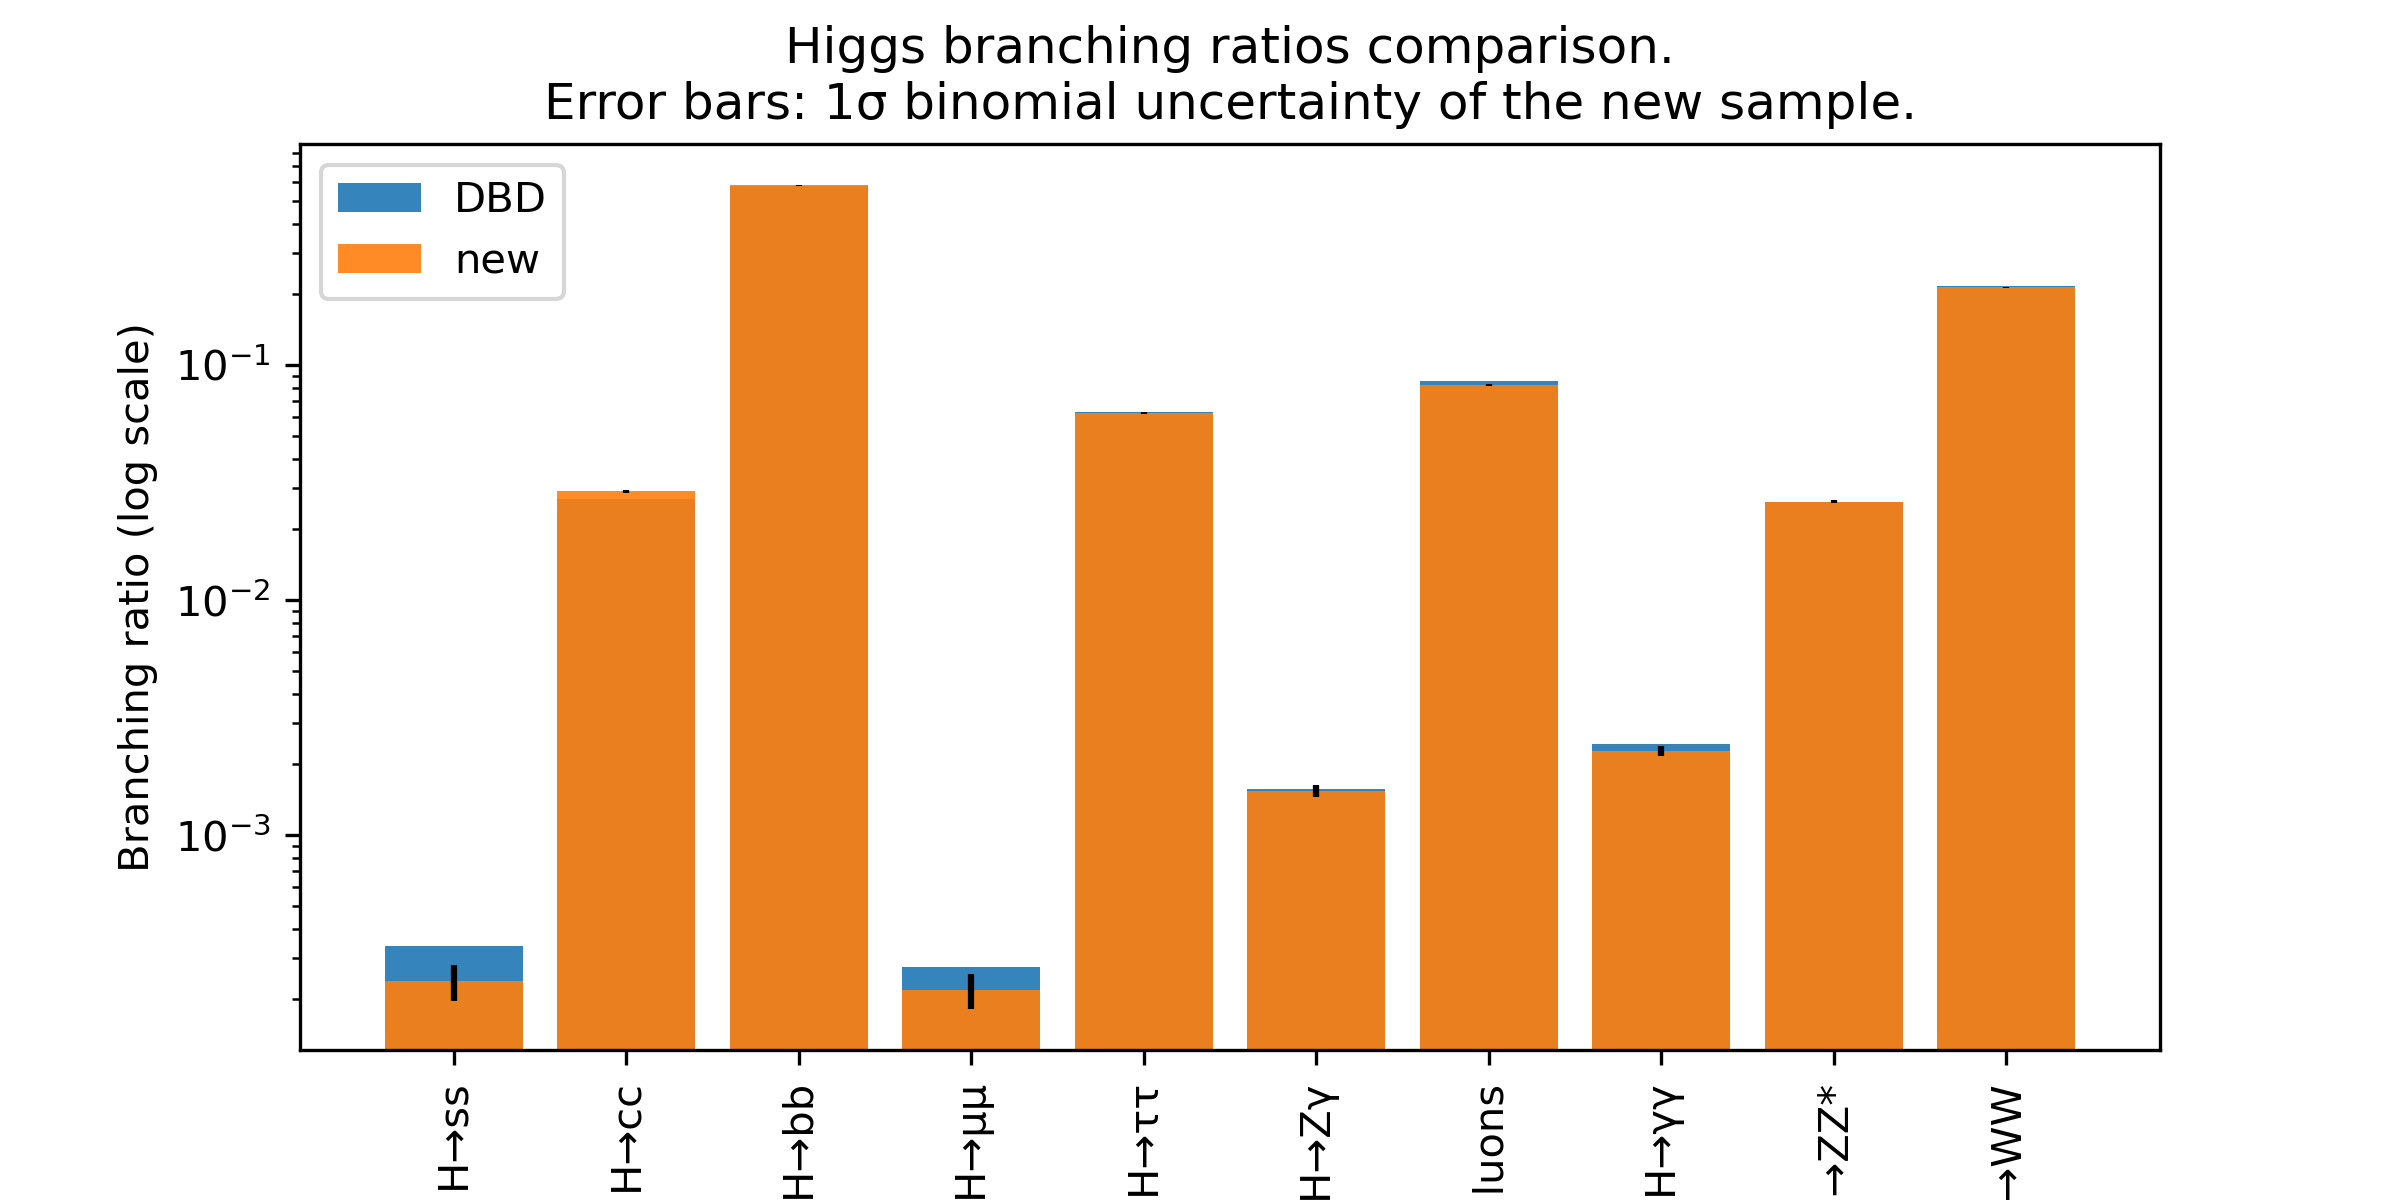
\includegraphics[width=.8\textwidth, keepaspectratio]
    {branching_ratio_difference_log}
  \end{column}
  \begin{column}{0.5\textwidth}
  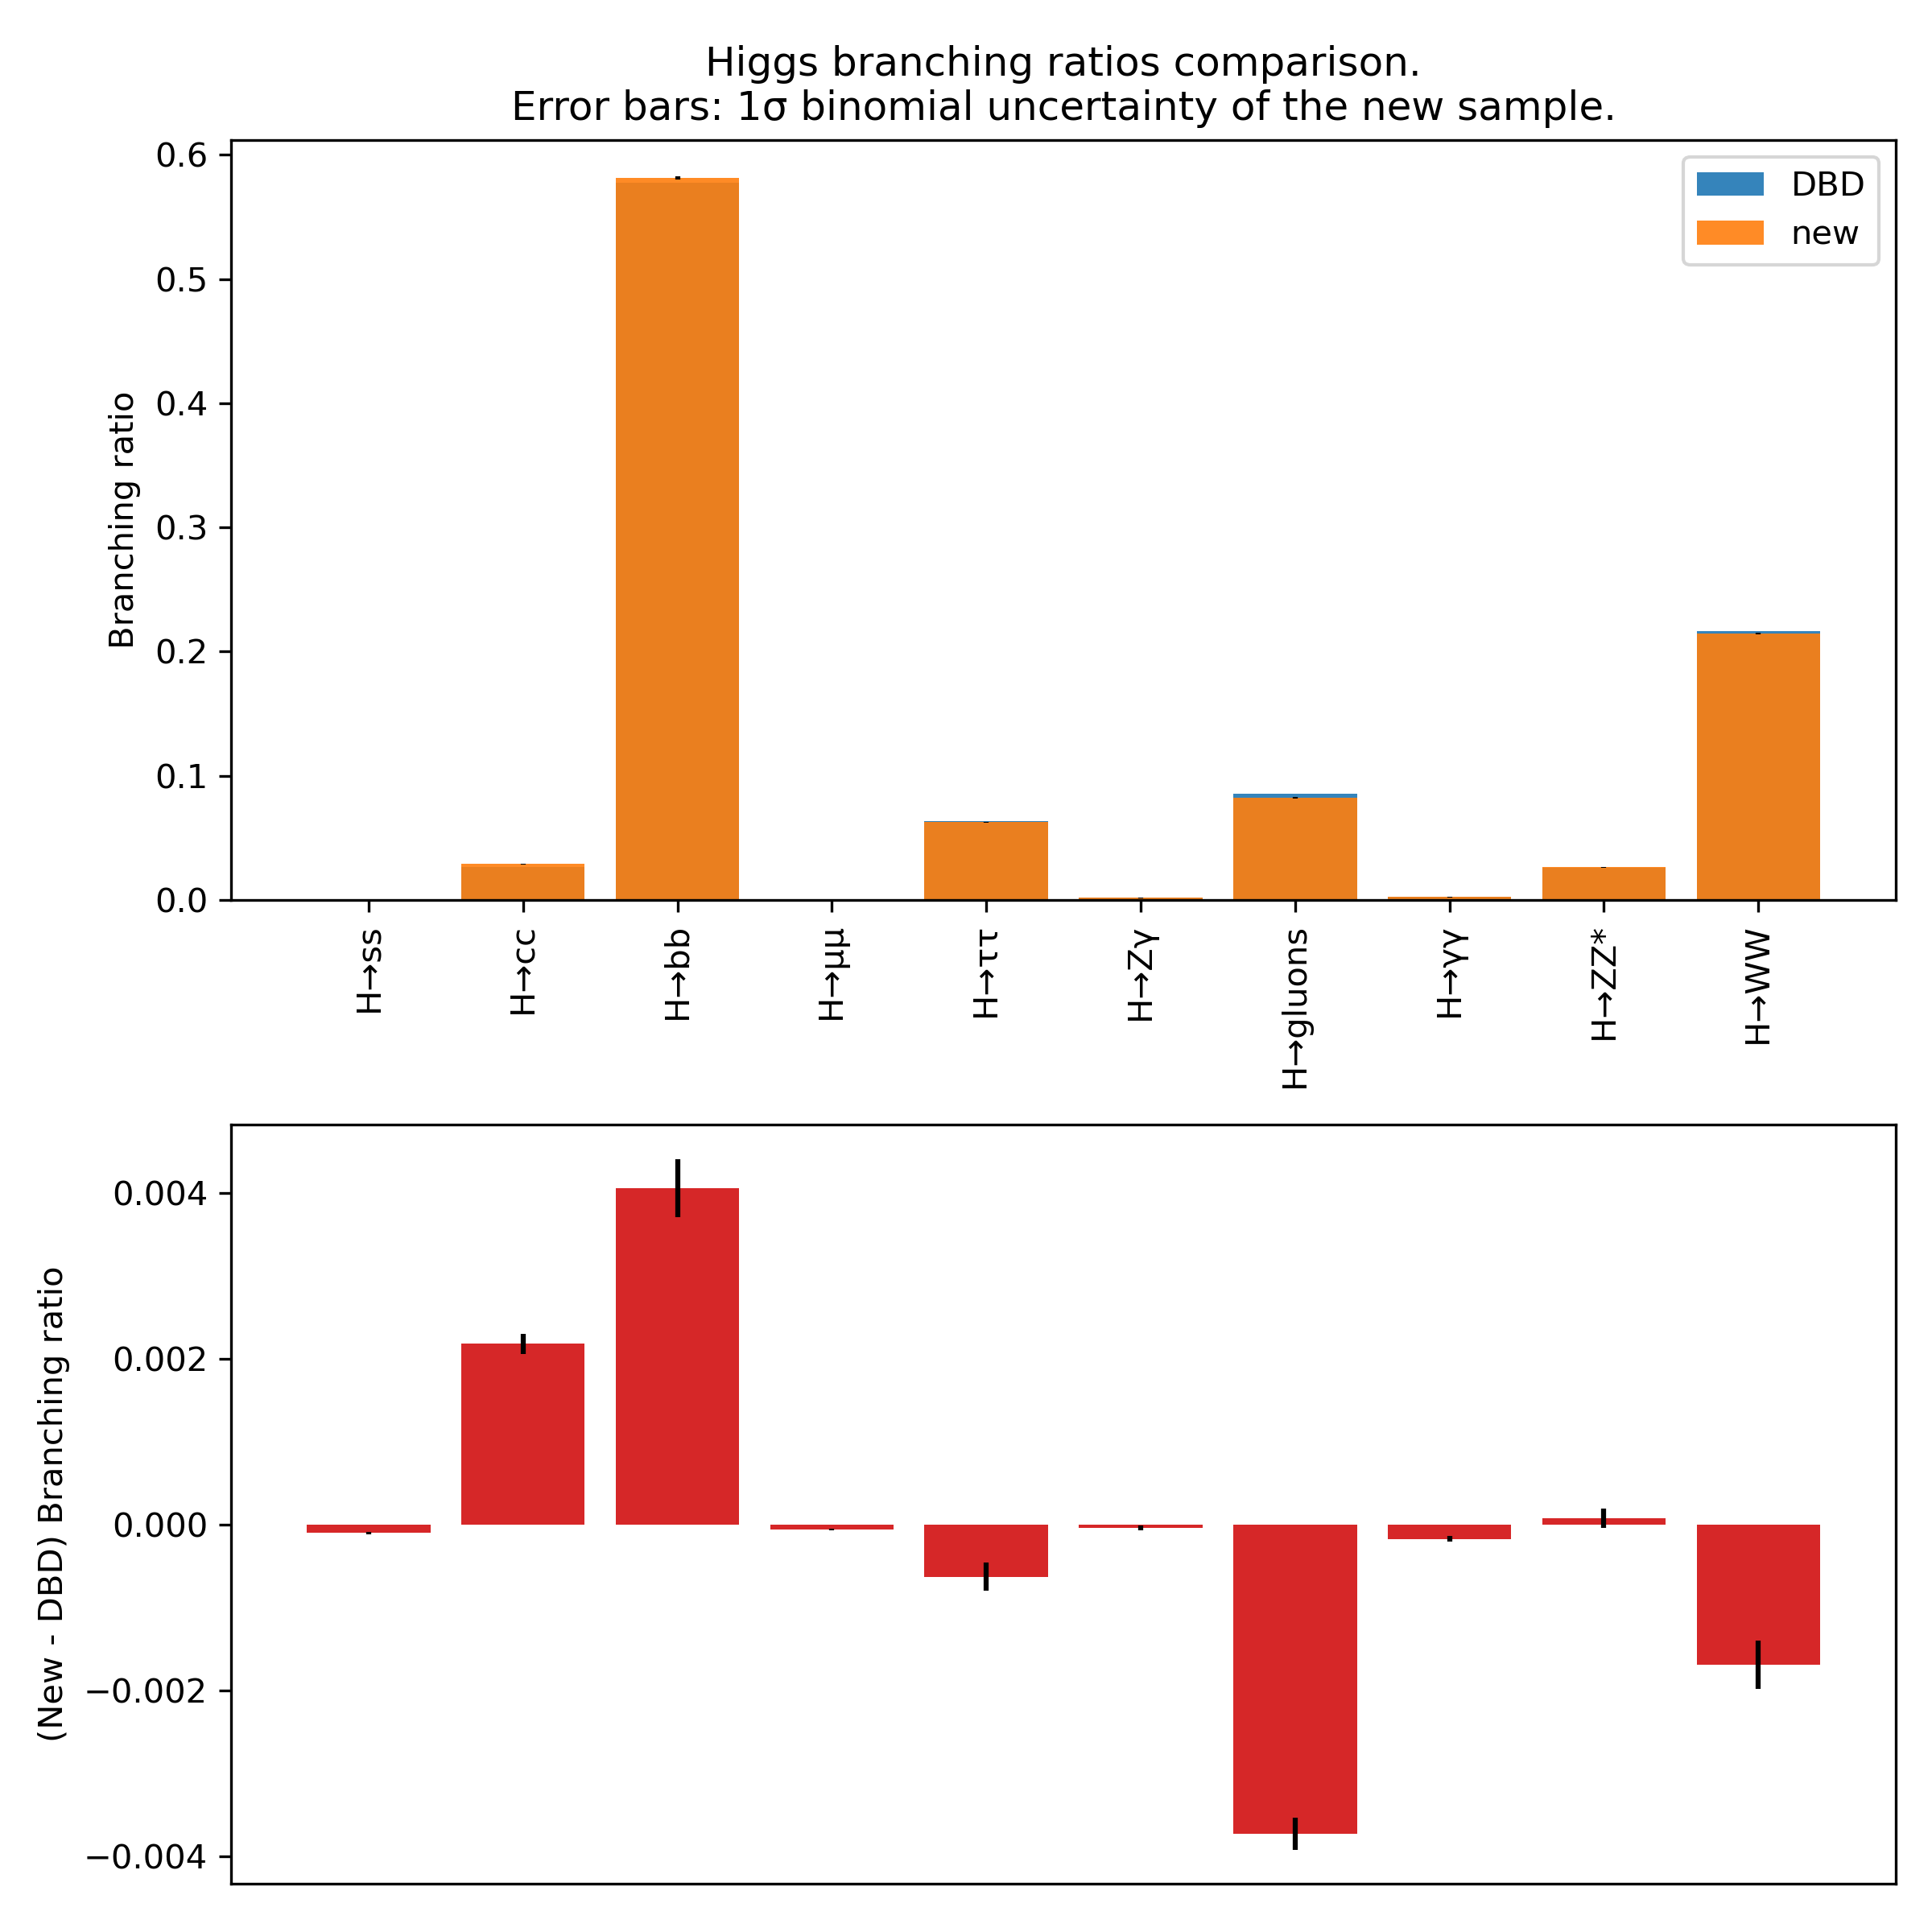
\includegraphics[width=.8\textwidth, keepaspectratio]
    {branching_ratio_difference}
  \end{column}
  \end{columns}
  \end{frame}

\begin{frame}
  \frametitle{\#PFOs per Higgs decay mode}
  Increased overlay makes it harder to use \textit{global} information.
  \begin{center}
  \only<1>{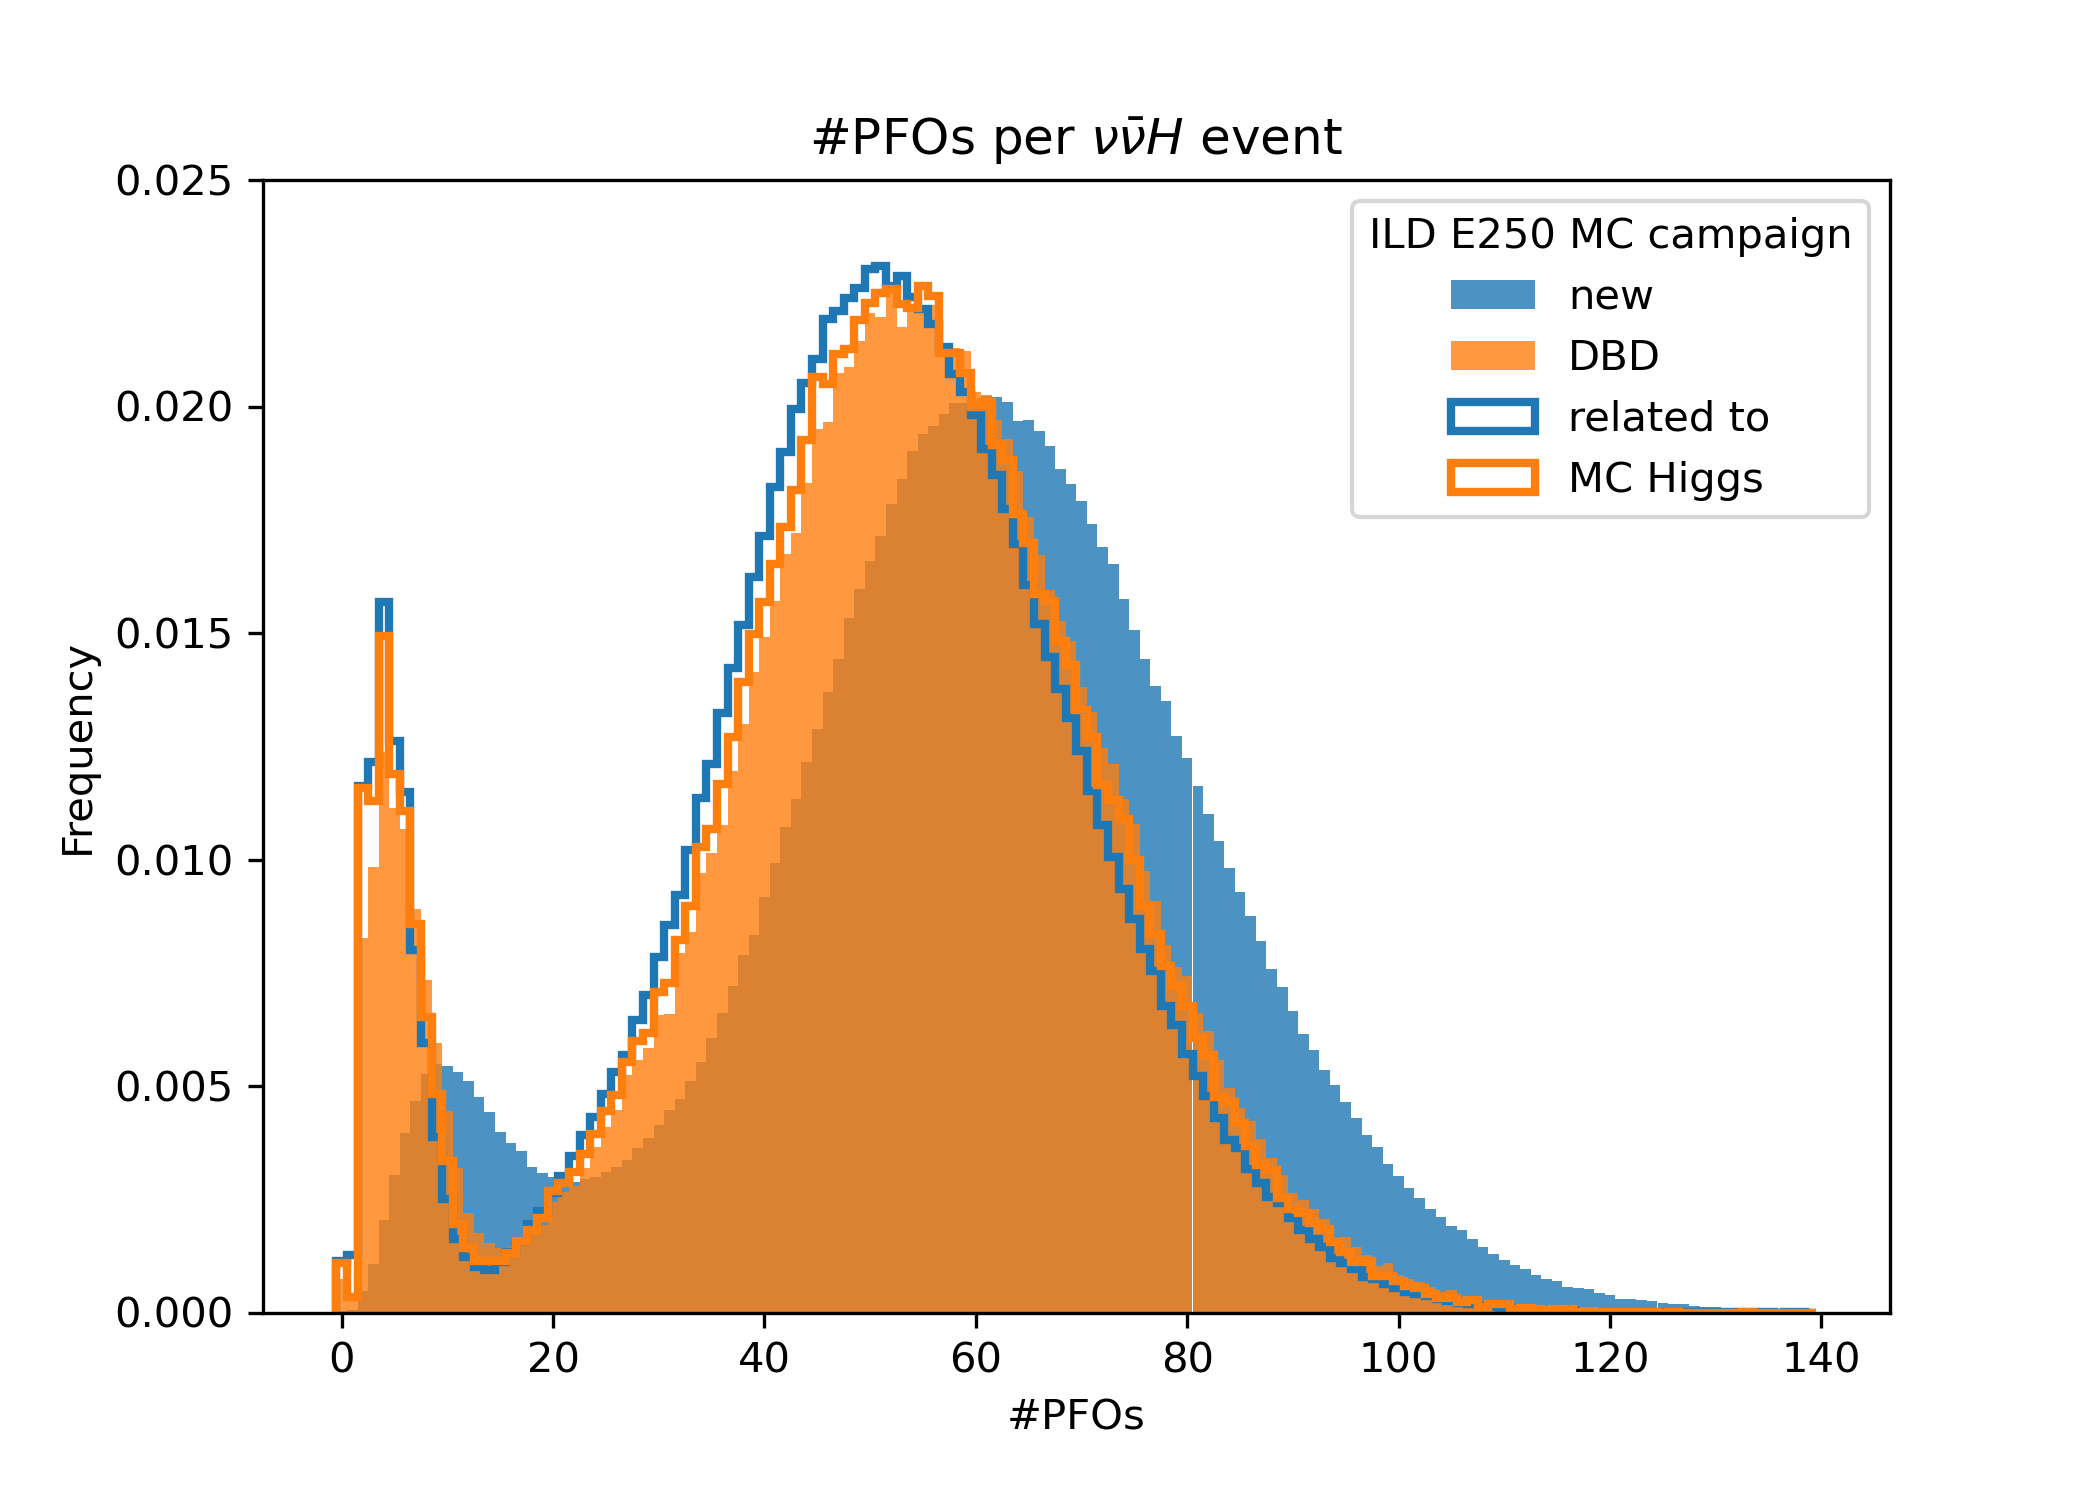
\includegraphics[height=0.8\textheight, width=\textwidth, keepaspectratio]
      {n_pfos_full_and_only_higgs}}
      \only<2->{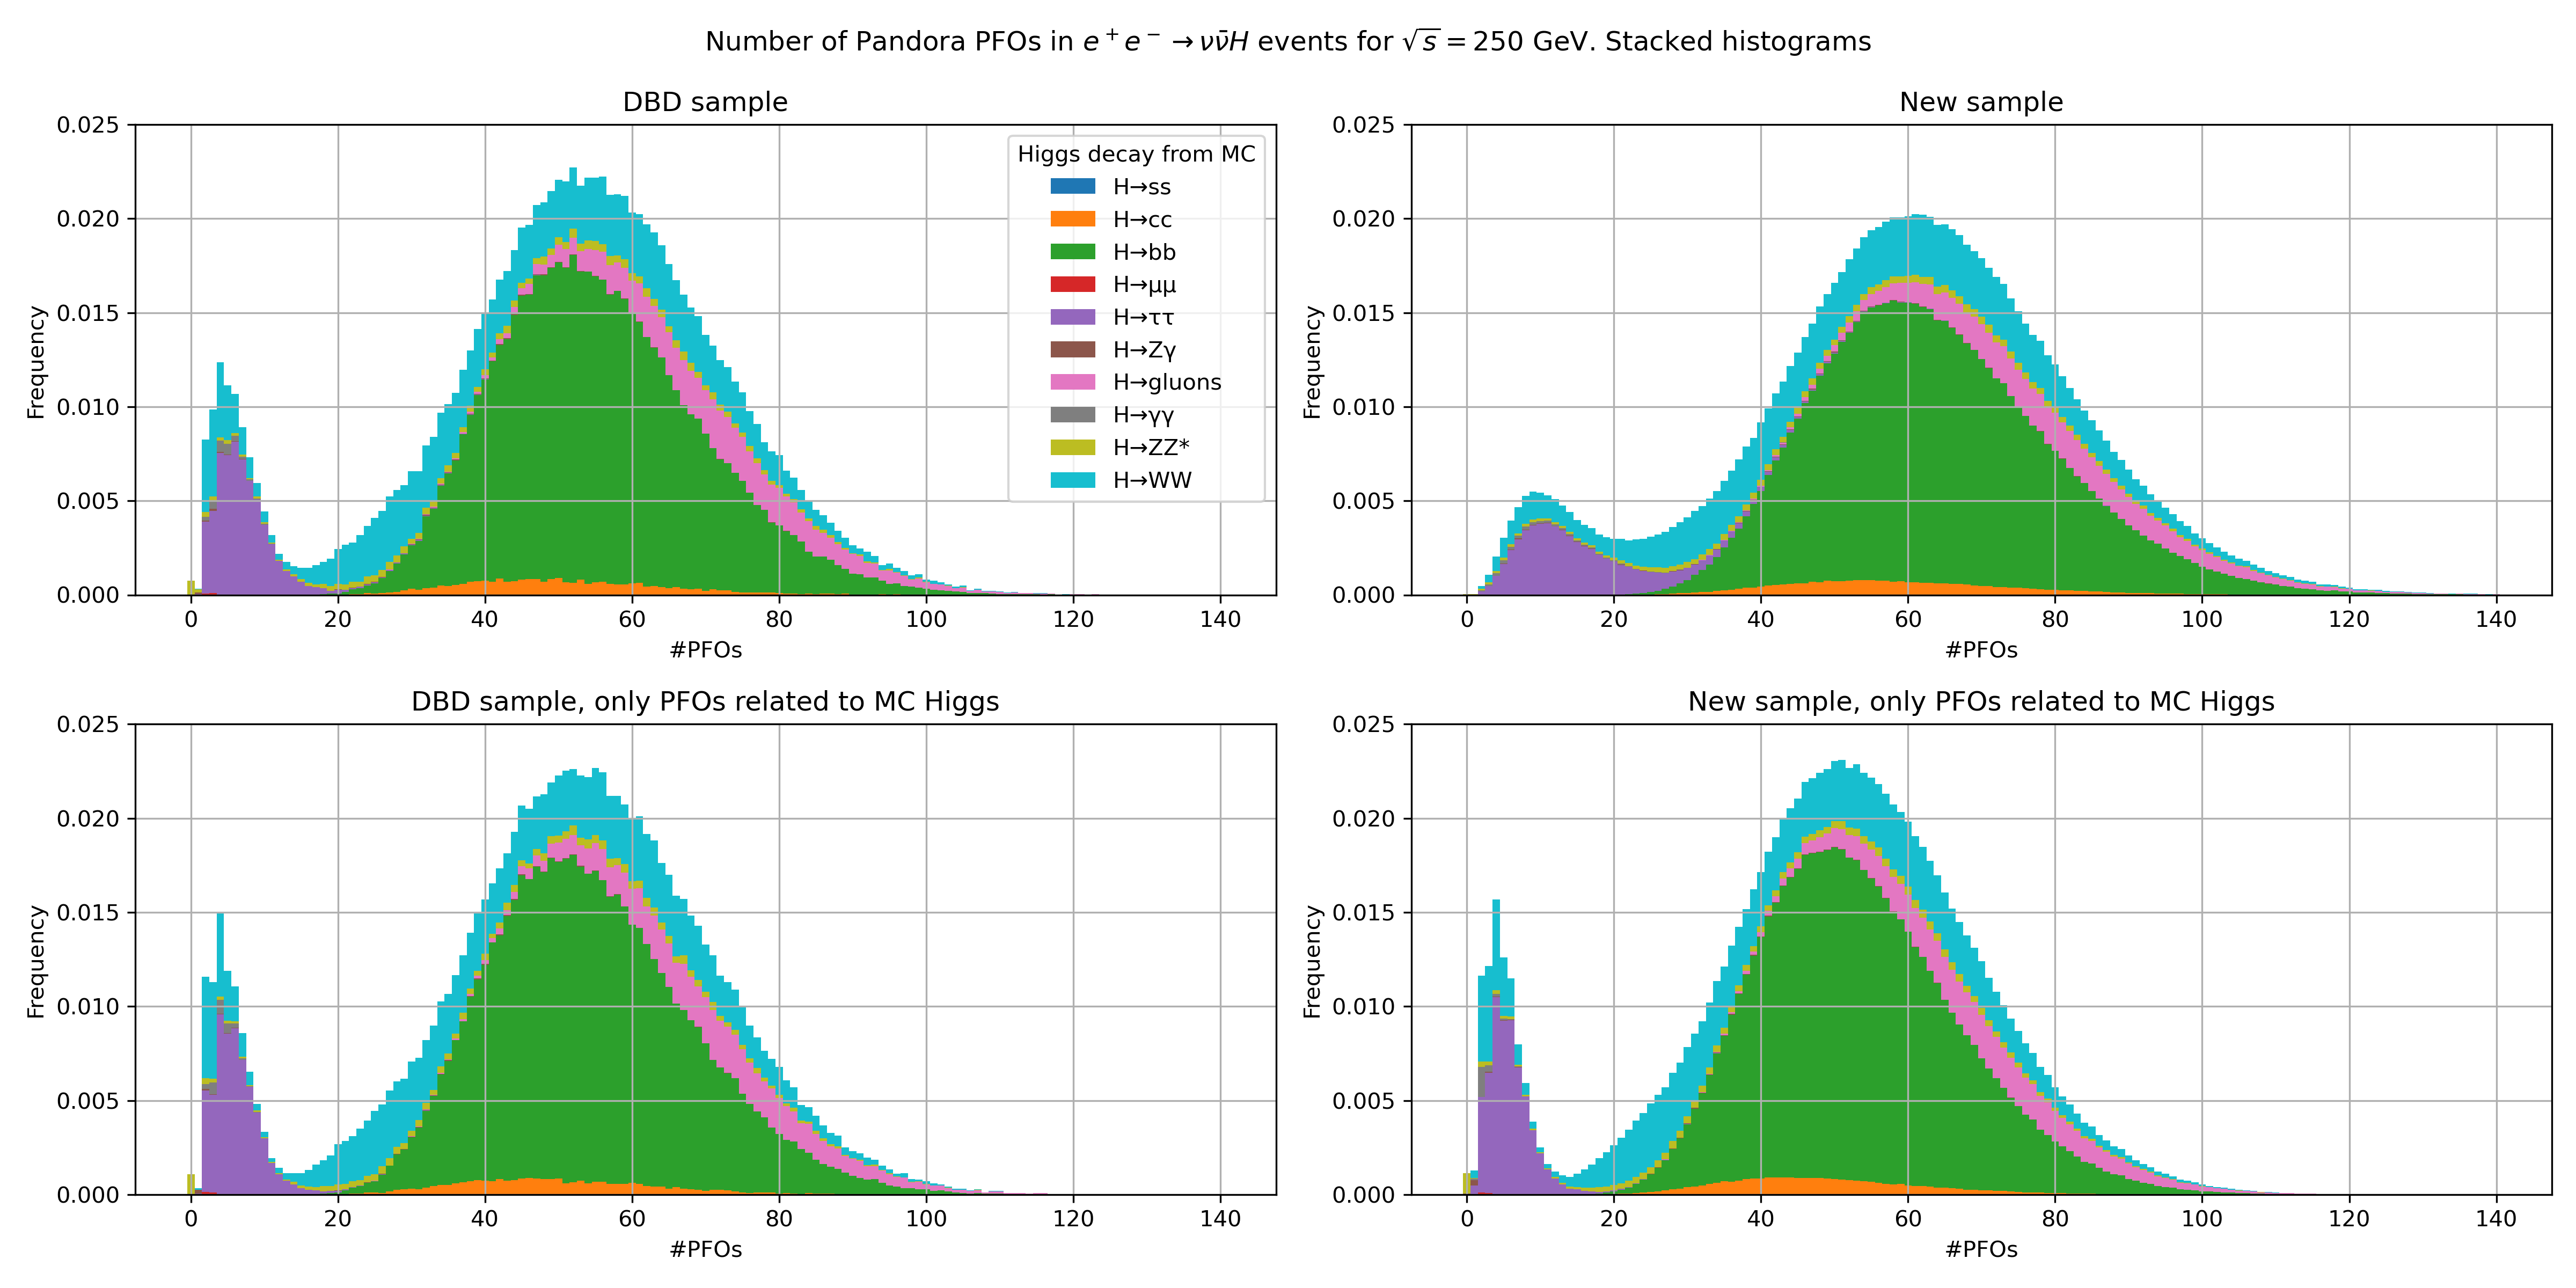
\includegraphics[height=0.8\textheight, width=\textwidth, keepaspectratio]
        {decays_stacked_n_pfos}}
  \end{center}
  \end{frame}
  \xsection{myblue}{Conclusion}


\begin{frame}
  \frametitle{Conclusion}
  \begin{itemize}
    \item[+] Smoother distributions due to increased sample size.
    \item[+] Reconstruction of the Higgs boson itself is comparable.
    \item[--] Overlay should not be ignored (any more) by me:
    \begin{itemize}
        \item Replace \textit{global} variables by a more local version
            (e.g. \texttt{\#PFOs}~$\rightarrow$~\texttt{\#PFOs in fat jet(s)}) \textit{or}
        \item Have a customized, stricter particle definition that reduces the
            overlay within the analysis \textit{and/or}
        \item Adapt the selection cuts and retrain the MVA tools.
    \end{itemize}
    \item[!] Many thanks to all who are involved in providing the (new) samples!
  \end{itemize}
  \end{frame}
  \newcounter{finalframe}
\setcounter{finalframe}{\value{framenumber}}

\xsection*{myblue}{Back-up}[pr_ilc_cavity_resized]

\begin{frame}
  \frametitle{Two types of variables}
  It is important to assign each observed momentum to the right parent particle.
  \begin{columns}[c,onlytextwidth]
  \begin{column}{0.5\textwidth}
  \begin{block}{Higgs-only variables}
  \begin{itemize}
    \item E.g. $M_H^{\tn{vis}}$, recoil to $M_H^{\tn{vis}}$.
    \item But also \textbf{number of charged hadrons}.
    \item Differ between the Higgs decay modes.
    \item Same distr. for all four $Z\rightarrow l \bar{l}$ samples.
    \item Distributions taken from the \textit{reference sample}.
  \end{itemize}
  \end{block}
  \end{column}
  \begin{column}{0.5\textwidth}
  \begin{block}{Z-only variables}
  \begin{itemize}
    \item E.g. $M_{\tn{recoil}}$, $M_Z$.
    \item C.f. recoil mass technique.
    \item Independent of the Higgs boson decay (model).
    \item Distributions taken from Monte Carlo (MC) generated data.
  \end{itemize}
  \end{block}
  \end{column}
  \end{columns}
  \end{frame}

\begin{frame}
  \frametitle{Two types of samples}
  \begin{columns}[c,onlytextwidth]
  \begin{column}{0.5\textwidth}
  \begin{block}{Counting sample}
  \begin{itemize}
    \item Count the number of events in the samples.
    \item Three samples are built:
        $Z\rightarrow e^+ e^-$, $\tau^+ \tau^-$ and $\nu_l \bar{\nu}_l$.
    \item Event selection based on both Z-only and Higgs-only variables.
    \item Z-only selection efficiency from MC.
    \item Higgs-only sel. eff. from reference sample.
  \end{itemize}
  \end{block}
  \end{column}
  \begin{column}{0.5\textwidth}
  \begin{block}{Reference sample}
  \begin{itemize}
    \item Extract the fraction of events passing a (Higgs-only) selection.
    \item Employed Higgsstrahlung events: $Z\rightarrow \mu^+ \mu^-$.
    \item Event selection based on just the Z-only variables.
    \item Selection efficiency from MC. \\ {\color{white} X}
  \end{itemize}
  \end{block}
  \end{column}
  \end{columns}
  \end{frame}

\begin{frame}<100>
  \frametitle{Uncertainty on the \texorpdfstring{{$\nu\bar{\nu}H$}}{vvH} cross section}
  \begin{align*}
    \sigma_{\nu\bar{\nu}H} &= \frac{N_{\nu\bar{\nu}H}}{L}
        = \frac{N_{\nu\bar{\nu}H}}
               {BR(Z\rightarrow \nu\bar{\nu})\epsilon_Z^{\mu, e} \epsilon_H L}
    \\
    \frac{ \Delta\sigma_{\nu\bar{\nu}H} }{ \sigma_{\nu\bar{\nu}H} }
    &\approx \sqrt{ \left( \frac{ \Delta N_{\nu\bar{\nu}H} }
                                { N_{\nu\bar{\nu}H}} \right)^2
                 +  \left( \frac{ \Delta \epsilon_H }{ \epsilon_H} \right)^2 }
    \\
    &= \sqrt{ \frac{ D_{\nu\bar{\nu}H} }{ (N_{\nu\bar{\nu}H})^2 }
            + \frac{ D_{Z}^{\mu, e} }{ (N_{Z}^{\mu, e})^2 }
            + \frac{ D_{H|Z}^{\mu, e} }{ (N_{H|Z}^{\mu, e})^2 }
            - \frac{ 2 D_{H|Z}^{\mu, e} }{ N_{H|Z}^{\mu, e} N_{Z}^{\mu, e} } }
    \end{align*}
    Includes the systematic uncertainty from the selection
    (e.g. cut on $N_{\tn{ch. hadr.}}$). \\
    Assumption: Background distributions well known. \\
  \end{frame}

\begin{frame}<100>
  \frametitle{The \texorpdfstring{$\nu\bar{\nu}H$}{vvH} BDT}
  Up to now trained an XGBoost BDT with the DBD MC samples.
  The criterium for the variables is to:
  \begin{columns}[c,onlytextwidth]
  \begin{column}{0.5\textwidth}
  \begin{block}{Only use Higgs boson remnants, nothing from the recoiling Z boson}
  \begin{itemize}
    \item[+] $\delta\sigma_{H\nu\bar{\nu}}\approx3.1\%$ achieved so far.
    \item N$_{\tn{charged hadrons}}$, N$_{\tn{neutral hadrons}}$, N$_\gamma$,
        N$_e$, N$_\mu$, N$_{\tn{isolated leptons}}$.
    \item M$_{\tn{Higgs}}$(=M$_{\tn{vis}})$, M$_{\tn{Higgs-recoil}}$,
        cos$(\theta_{\tn{miss}})$.
    \item principle thrust, z-component of thrust axis, major thrust,
        minor thrust, sphericity, aplanarity,
        E$^{\tn{max}}_{\tn{isolated lepton}}$,
        cos$(\theta_{\tn{isolated lepton}})$.
  \end{itemize}
  \end{block}
  \end{column}
  \begin{column}{0.5\textwidth}
  \begin{block}{and indep. of the Higgs production (WW-fusion, Higgsstrahlung).}
  \begin{itemize}
    \item[+] $\delta\sigma_{H\nu\bar{\nu}}\approx3.8\%$ achieved so far.
    \item N$_{\tn{charged hadrons}}$, N$_{\tn{neutral hadrons}}$, N$_\gamma$,
        N$_e$, N$_\mu$, N$_{\tn{isolated leptons}}$.
    \item M$_{\tn{Higgs}}$(=M$_{\tn{vis}})$.
    \item[]
    \item[]
    \item[]
    \item[]
  \end{itemize}
  \end{block}
  \end{column}
  \end{columns}
  \end{frame}

\begin{frame}<100>
  \frametitle{The \textbf{ILD DBD} 250~\GeV data set}
  \begin{columns}[T,onlytextwidth]
  \begin{column}{0.5\textwidth}
  \begin{table}
    \resizebox{\textwidth}{!}{
    \InputTable{tab_mctabularUsedOppositePol.tex}
    }
  \end{table}
  \end{column}
  \begin{column}{0.5\textwidth}
  \vspace{0.05\textheight} % To have the text stay below the logo.
  \begin{itemize}
    \item Large Standard Model event generation and detector simulation.
    \begin{itemize}
      \item[$\rightarrow$] for Detailed Baseline Design (DBD).
    \end{itemize}
    \item A particle flow algorithm (PandoraPFA) was run on simulated events in 2013.
    \item Process luminosities between $\sim 20~$fb$^{-1}$ (Bhabha)
        and 1000~fb$^{-1}$ (Higgs).
  \end{itemize}
  \end{column}
  \end{columns}
  \end{frame}

\setcounter{framenumber}{\value{finalframe}}
\end{document}